% -----------------------------------------------------------------------
% Python Tutorial
% WS 18/19
% -----------------------------------------------------------------------
\documentclass[enabledeprecatedfontcommands, fontsize=12pt,
     open=right, a4paper,
     twoside, DIV=11,
     abstractoff,
     headsepline,
     numbers=noenddot,
     BCOR=15mm,
     headings=standardclasses,
     headings=big]{scrbook}
\KOMAoptions{cleardoublepage=empty}
% Header f�r Variablen
% Variablen
\newcommand{\theSemester}{Sommersemester 2019}
% Variable f�r die Vorlesung
\newcommand{\theProject}{}
% Variable f�r den Studiengang
\newcommand{\theTitle}{Python}
% Variable f�r den Hochschul-Namen
\newcommand{\theSchool}{Hochschule Kaiserslautern}
% Variable f�r den Dozenten
\newcommand{\theAuthor}{
    Julian  Bernhart,
    Manfred Brill,
    Eric Brunk,
    Mathias Fedder,
    Christopher Gross,
    Robin Guth,
    Rainer Haffner,
    Matthias Haselmaier,
 %   Kathrin Hentschel,
    Fabian Kalweit,
    Lukas Kuhn,
    Kevin Konrad,
    Philipp Lauer,
    Miriam Lohm�ller,
    Sebastian Morsch,
    Anatoli Sch�fer,
    Denis Schlusche,
    Christoph Seibel,
    Marc Zintel
    Marc Heinrich
}

%
% ----------------------------------------------------------------------------------------------
% Vorlage für Dokumentation auf LaTeX-Basis im Projekt InfoStuDi
% --------------------------------------------------------------------------------------------
% utf-8 verwenden, aber der Vorlage vorgaukeln, ansinew würde verwendet werden. Quick-fix um mit
% Manfred Brills mb.sty kompatibel zu sein
\makeatletter
\newcommand{\dontusepackage}[2][]{%
  \@namedef{ver@#2.sty}{9999/12/31}%
  \@namedef{opt@#2.sty}{#1}}
\makeatother
\usepackage[utf8]{inputenc}
\dontusepackage[ansinew]{inputenc}
\usepackage{mb}
\usepackage{mbmath}
\usepackage{textcomp}
% Array-Paket für mehr Kontrolle der Tabellen
\usepackage{array}
% ifthen für Ein- und Ausblenden der Lösungen.
\usepackage{ifthen}
% Paket für Postscript Pi-Fonts
\usepackage{pifont}
% PSTricks
%\usepackage{pstricks}
% Paket für das einfache Umdefinieren von Listen
\usepackage[shortlabels]{enumitem}
% Alphabetischer Index
\usepackage{imakeidx}
\makeindex[title=Index,columns=2,options=-s german,intoc]
% Header und Footer mit KomaScript
\usepackage[automark, headsepline]{scrlayer-scrpage}
%
% Header für Werkzeuge, Begriffe aus dem Software-Management
\input{variablen}
% Farben
\input{colors}
% Koordinatensysteme und andere Makros
\input{coordinateSystems}
% Standardverzeichnis für das Basisverzeichnis der Bilder
%
\newcommand{\imagePath}{./images}
%
\raggedbottom
\setlength{\parskip}{2.0ex}
\setlength{\parindent}{0.0cm}
%% Verhindert Schusterjungen und Hurenkinder
\clubpenalty = 10000
\widowpenalty = 10000 \displaywidowpenalty = 10000
%
\setcounter{secnumdepth}{2}
\setcounter{tocdepth}{2}
%
\pagestyle{scrheadings}
\clearscrheadfoot
% Thema des Dokuments in die Kopfzeile
\ihead{\headmark}
\ohead[]{\pagemark}
\chead{}
\pagestyle{scrheadings}
% Abstände zwischen Caption und Bild/Tabelle
\setlength\abovecaptionskip          {0.4em}
\setlength\belowcaptionskip          {0.2em}
% Anteil der Grafiken höher auf jeder Seite!
\renewcommand{\textfraction}{0.001}
\renewcommand{\topfraction}{0.99}
% Literatur-Stil
\bibliographystyle{geralpha}
% Listingspaket
\usepackage{listings}
\lstloadlanguages{Java}
\lstset{language=Java}
\definecolor{lstback}{gray}{0.85}
\lstset{backgroundcolor=\color{lstback}}
\lstset{extendedchars=true}
\lstset{showstringspaces = false}
\lstset{basicstyle = \ttfamily \small}
%% listings mit listings.sty
%
% Kommando für den Flattersatz bei nebeneinander liegenden Abbildungen
\newcommand{\flatter}{\setlength{\rightskip}{0pt plus 2cm}}
%
% Schritte in einer Aufzählung, dafür einen Zähler (schritt) und die Umgebung
% schritte definieren.
\newcounter{schritt}
\newenvironment{schritte}%
{\begin{list}%
{Schritt \arabic{schritt}:}%
{\usecounter{schritt}\settowidth{\labelwidth}{Schritt 1:}%
\setlength{\leftmargin}{\labelwidth}\addtolength\leftmargin{\labelsep}%
\parsep0.0ex\partopsep-0.3ex\itemsep2pt\topsep0.0ex}}{\end{list}}
% Dateinamen für interne Musterlösungen
\newcommand{\filename}[1]{%
\ifthenelse{\boolean{solutions}}{\framebox[50mm]{\parbox{40mm}{\textbf #1}}\vspace{6pt}}{}}
%   Taste
\newcommand{\taste}[1]{\small\textsf{#1}\normalsize}
%   geschützte Namen (NICHT in chapter, section usw. verwenden!)
\newcommand{\name}[1]{\textsl{#1}}
%   Fachbegriffe/Erklärung von Abkürzungen
\newcommand{\begriff}[1]{\index{#1}\textit{#1}}
%
\newcommand{\algorithmus}[2]{%
\vspace{4pt}\fboxsep 1mm \framebox[140mm]
{\parbox{135mm}{{\textbf{#1}}\vspace{2pt}#2}}\vspace{4pt}}
%
%   Dateinamen/Pfade
\newcommand{\datei}[1]{\texttt{#1}\normalsize}
%   Tip (in einer Box)
\newcommand{\tip}[1]{%
\vspace{4pt}\fboxsep 1mm \framebox[140mm]
{\parbox{135mm}{{\textbf{Tipp}}:\\ #1}}\vspace{4pt}}
%
%   Reflektion (in einer Box)
%
\newcommand{\reflection}[1]{
\begin{quote}\fboxsep 3mm\framebox[140mm][c]{\parbox{130mm}{{\textbf{Reflektion}:\\}#1}}\end{quote}}
%
%   Angabe, was die Studierenden lesen sollen (in einer Box)

\newcommand{\lesen}[1]{%
\begin{minipage}[c]{2.5cm}
\centering
\includegraphics[width=2cm]{\imagePath/Misc/buchicon}%
\end{minipage}%
\begin{minipage}[t]{12cm}%
#1%
\end{minipage}}
%
%   Angabe im Begleittext, was die Studierenden lesen sollen (in einer Box)
%   Dieses Icon wird für Angaben verwendet, die nicht verpflichtend zu lesen
%   sind. Also "nice-to-have", "wenn sie noch Zeit haben".
\newcommand{\vertiefen}[1]{%
\begin{minipage}[b]{2.5cm}
\centering
\includegraphics[width=2cm]{\imagePath/Misc/reading}%
\end{minipage}%
\begin{minipage}[b\newcommand{\firefox}{\texttt{Mozilla Firefox}}
\newcommand{\kde}{\texttt{KDE}}]{12cm}%
#1%
\end{minipage}}
%
% Jetzt kommt die Definition der Kontrollfrage; die Nummerierung
% für das ganze erhalten wir mit Hilfe von \item{\kontroll}.
%
% Ein Counter für die Kontrollfragen. Wir zählen diesen Counter selbst hoch
% mit einem entsprechenden Kommando, das wir in \item verwenden.
% 1
\newcounter{kontrollCounter}[section]
\newcommand{\kontroll}[0]{
    \refstepcounter{kontrollCounter}
    % Kapitelnummer.Zähler für das Item
    \arabic{chapter}.\arabic{kontrollCounter}
    % Das Label ist bis auf weiteres "kontrolle:Kapitelnummer:kontrollcounter
    \label{kontrolle:\arabic{chapter}:\arabic{kontrollCounter}}
}
% Jetzt kommt die Definition der Kontrollfrage; die Nummerierung
% für das ganze erhalten wir mit Hilfe von \item{\kontroll}.
\newcommand{\kontrollfrage}[1]{%
\begin{minipage}[c]{1.85cm}
\huge{\ding{46}}%
\end{minipage}%
\begin{minipage}[t]{12cm}%
\begin{itemize}#1%
\end{itemize}%
\end{minipage}}
%
% Einblenden von Musterlösungen
%
% Schalter für das ein- und ausblenden der Lösungen
\newboolean{solutions}
%
% Theorem-Umgebung für die Übungsaufgaben
% Wichtig: alle Attribute einstellen, dann die neue
% theorem-Umgebung mit newtheorem definieren!
% Oder, wie hier, durch das Einschließen in {}
%
{
% Zeilenumbruch bei Aufgaben-Überschrift
\theoremstyle{break}
% "Normaler" Font im Text
\theorembodyfont{\normalfont}
% Kapitelweise neu nummerieren
% 2
\newtheorem{auftitle}{Aufgabe}[section]
}
%
% Definition für die Kennzeichnung der Übungsaufgaben
%
\newcommand{\uebung}{%
\vspace*{11pt}%
\begin{tabular}{@{}p{2.25cm}@{}p{11.7cm}}%
\huge{\ding{45}}&\Large{\textbf{Übungsaufgaben}}%
\end{tabular}%
}
% Ein Counter für die Übungsaufgaben. Wir zählen diesen Counter selbst hoch
% mit einem entsprechenden Kommando, das wir in \item verwenden.
% 3
\newcounter{aufgabenCounter}[section]
\newcommand{\auf}[0]{
    \refstepcounter{aufgabenCounter}
    % Kapitelnummer.Zähler für das Item
    \arabic{chapter}.\arabic{aufgabenCounter}
}
% Der Text der Aufgaben steht im Ordner ../Uebungsaufgaben/aufgaben/aufgabenstellungen,
% so können wir die Dateien aus der Veranstaltung
% Wahrscheinlichkeitsrechnung und Statistik verwenden; und die neuen
% Aufgaben gehen in den allgemeinen Fundus ein.
%

% Umgebungen für Satz, Definition, Beweis, ... . Wir orientieren uns am Mathematik-Buch,
% dort gab es diese Umgebungen auch schon. Im Grunde sind das einfach
% wieder theorem-Umgebungen.
{
\setlength\theorempreskipamount{5pt plus 3pt minus 1.5pt}
\setlength\theorempostskipamount{5pt plus 1pt minus 1pt}
% "Normaler" Font im Text
\theorembodyfont{\normalfont}
% Die Namen sind so gewählt, dass sie kompatibel zu Beamer sind; dann können
% wir den Text aus Folien kopieren und umgekehrt auch.
% 4
\newtheorem{Satz}{Satz}[section]
\newtheorem{Fakt}{Fakt}[section]
\newtheorem{Definition}{Definition}[section]
}
%
{
\setlength\theorempreskipamount{8pt plus 3pt minus 1.5pt}
\setlength\theorempostskipamount{5pt plus 1pt minus 1pt}
\theoremstyle{break}
% "Normaler" Font im Text
\theorembodyfont{\normalfont}
\newtheorem{datensatz}{Datensatz}
}
% Text mit Pfad
\newcommand{\aufgabentext}[1]{\renewcommand{\labelenumi}{\alph{enumi})}\auftitle\label{#1}\input{../../uebungsaufgaben/Stochastik/aufgaben/aufgabenstellungen/#1}}
% Funktion für die Lösungs-Hinweise für eine Aufgabe. Der Text
% steht analog zu den Übungsaufgaben im Ordner aufgaben/loesungen.
\newcommand{\hinweistext}[1]{\renewcommand{\labelenumi}{\alph{enumi})}\input{../../Uebungsaufgaben/Stochastik/aufgaben/loesungen/#1}}
% Und jetzt die Funktionen, die wir im Text aufrufen
\newcommand{\aufgabe}[1]{\aufgabentext{#1}}
% Lösungshinweise im Anhang
\newcommand{\hinweis}[1]{\subsubsection*{Aufgabe \ref{#1}} \hinweistext{#1}}
%
% Datensatz-Texte und Daten in eigener Datei
\newcommand{\dataset}[1]{\begin{datensatz}\label{#1}\input{../../Uebungsaufgaben/Stochastik/datasets/#1}\end{datensatz}}
% Teilaufgaben alphabetisch nummerieren
\renewcommand{\labelenumi}{\arabic{enumi})}
%
% Marginalien
%
\newcommand{\randnotiz}[1]{\marginpar{\small{\textbf{#1}}}}
%
% Gabelschlüssel als Marginalie und Hinweis auf Praxisbezug
\newcommand{\praxisbezug}[0]{\randnotiz{\includegraphics[width=1cm]{\imagePath/Misc/gabel}}}
%
% alert aus beamer-Folien zu emph machen
%
\newcommand{\alert}[1]{\emph{#1}}
%
%
\newcommand{\titelseite}[1]{%
% Titelseite
\pagenumbering{roman}%
\thispagestyle{empty}%
\begin{titlepage}%
% Volle Zeilenbreite verwenden!
\centering%
\vspace*{2cm}%

\Huge{#1}\\\vspace*{0.5cm}%

\vspace*{10cm}%

\Large{\theAuthor{}}%

\Large{\theProject{}}%

\Large{\theSchool{}}%
\end{titlepage}}

% Titelseite mit zusätzlicher Grafik
%
% Das obligatorische Argument ist der Titel des Dokuments.
% Als Default wird das Logo der Stochastik-Veranstaltung als Titelbild
% verwendet. Mit Hilfe eines optionalen Arguments kann
% ein anderes Bild verwendet werden!
% Beispiel: \titelseite[\imagePath/misc/ameise]{Das Liebesleben der Ameisen}
% Aufruf mit Standardbild:
% \titelseite{Das Liebesleben der Ameisen}
%
\newcommand{\titelseiteMitBild}[2][\imagePath/logos/python]{%
%% Titelseite
\pagenumbering{roman}%
\thispagestyle{empty}%
\begin{titlepage}%
% Volle Zeilenbreite verwenden!
\centering%
\vspace*{0.5cm}%

\Huge{#2}\\\vspace*{0.5cm}%

\vspace*{3.0cm}%
\includegraphics[height=6cm]{#1}%

\vspace*{3.0cm}%
\Large{\theAuthor{}}%

\Large{\theProject{}}%

\Large{\theSchool{}}%
\end{titlepage}}

%
% Schalter f�r das Ein- und Ausblenden der L�sungen
\setboolean{solutions}{true}
%
% Hyperref-Optionen für PDF-Files
% Dieses Paket muss als letztes eingebunden werden. Deshalb
% wird es hier "lokal" und nicht in setup.tex aufgeführt!
\usepackage[breaklinks]{hyperref}
\usepackage{breakurl}

\hypersetup{
pdftitle = {\theTitle},
pdfauthor = {\theAuthor},
pdfsubject = {},
pdfkeywords = {\theSchool},
pdfdisplaydoctitle = true,
pdfpagemode = UseThumbs,
colorlinks = false,
linkcolor = green,
linkbordercolor = {0 1 0},
pdfpagelayout = {SinglePage}
}

\urlstyle{same}

\listfiles
%
% Beginn Dokument
%
\begin{document}
\titelseiteMitBild{\theTitle{}}
%
% Vorwort
%
% !TeX root = ../pythonTutorial.tex
\chapter*{Vorwort}

Das vom Stifterverband gef�rderte Projekt \glqq Informatik studieren in der digitalen Gesellschaft (InfoStuDi)\grqq{}
erprobt und evaluiert neue Lehr-, Lern- und Pr�fungsformen in den Informatik-Studieng�ngen im Fachbereich Informatik und Mikrosystemtechnik der Hochschule Kaiserslautern.

Studieng�nge an einer Hochschule f�r
angewandte Wissenschaften bereiten die Studierenden auf die sp�tere Arbeitswelt vor.
Diese Arbeitswelt
wird von zeitlich und �rtlich ungebundenem T�tigkeiten gepr�gt sein.
Im Teilprojekt \glqq Collaborative Writing\grqq{} wurde eine neue Form einer Lehrveranstaltung erprobt,
die die Studierenden auf diese sp�tere Arbeitswelt vorbereiten soll.
Ein Team aus Studierenden und Lehrenden verfasst ein Dokument zu einem Thema der Informatik.
Dabei wird neben der Produktion von Texten auch Software entstehen.
Die Produktion des vorliegenden Dokuments
zum Thema Python wurde wie ein gro�es agiles Software-Projekt organisiert.
Drei Sprints wurden durchgef�hrt, das Team organisierte sich selbst. Werkzeuge wie \LaTeX{}, Git oder Jenkins wurden eingesetzt.
Die Studierenden waren nicht nur Autoren, sondern auch Fachlektoren, Software-Entwickler und f�r die Qualit�t des Gesamtergebnisses mit verantwortlich.

Dieses Projekt w�re nicht zustande gekommen ohne die Studierenden, die sich auf dieses Abenteuer im Rahmen der Lehrveranstaltung \glqq Aktuelle Themen aus Forschung und Praxis\grqq{} des Masterstudiengangs Informatik im Wintersemester~2018/19 eingelassen haben. An dieser Stelle ein herzliches \glqq Danke sch�n!\grqq{} f�r das Vertrauen und den Mut, sich auf diese Form einer
Lehrveranstaltung einzulassen.
Miriam Lohm�ller, als wissenschaftliche Mitarbeiterin im Projekt InfoStuDi t�tig, brachte ihre Erfahrung aus dem Verlagswesen ein und hat die von den Studierenden verfassten
Texte lektoriert. Fabian Kalweit, Mitarbeiter des Projektleiters im Fachbereich Informatik und Mikrosystemtechnik, hat das fachliche Lektorat unterst�tzt und insbesondere das Backend in GitHub
organisiert und gestaltet.

Der vorliegende Text stellt den Stand im M�rz 2019, nach Abschluss der Lehrveranstaltung, dar. Nat�rlich
ist das Python-Tutorial nicht abgeschlossen. Das komplette Projekt steht in Form eines �ffentlichen Git-Repositories (\cite{githubRepo})
zur Verf�gung und kann von interessierten Studierenden verwendet und vor allem weiterentwickelt werden.
Alle Autoren hoffen, dass unsere Leser den Text f�r gut befinden.

Die Texte wurden nach bestem Wissen und
Gewissen verfasst. Sollte der Text trotzdem Fehler enthalten, liegen diese in der alleinigen Verantwortung
des Projektleiters!

\vspace{\baselineskip}
\begin{flushright}\noindent
Zweibr�cken, im M�rz 2019\hfill

\hfill {\it Manfred  Brill}
\end{flushright}
\pagebreak
\section*{Das Team}
%Gruppenbild mit Dame -- das Team nach dem letzten Sprint Meeting am 31.~Januar~2019.

\begin{figure}[ht]
\centering
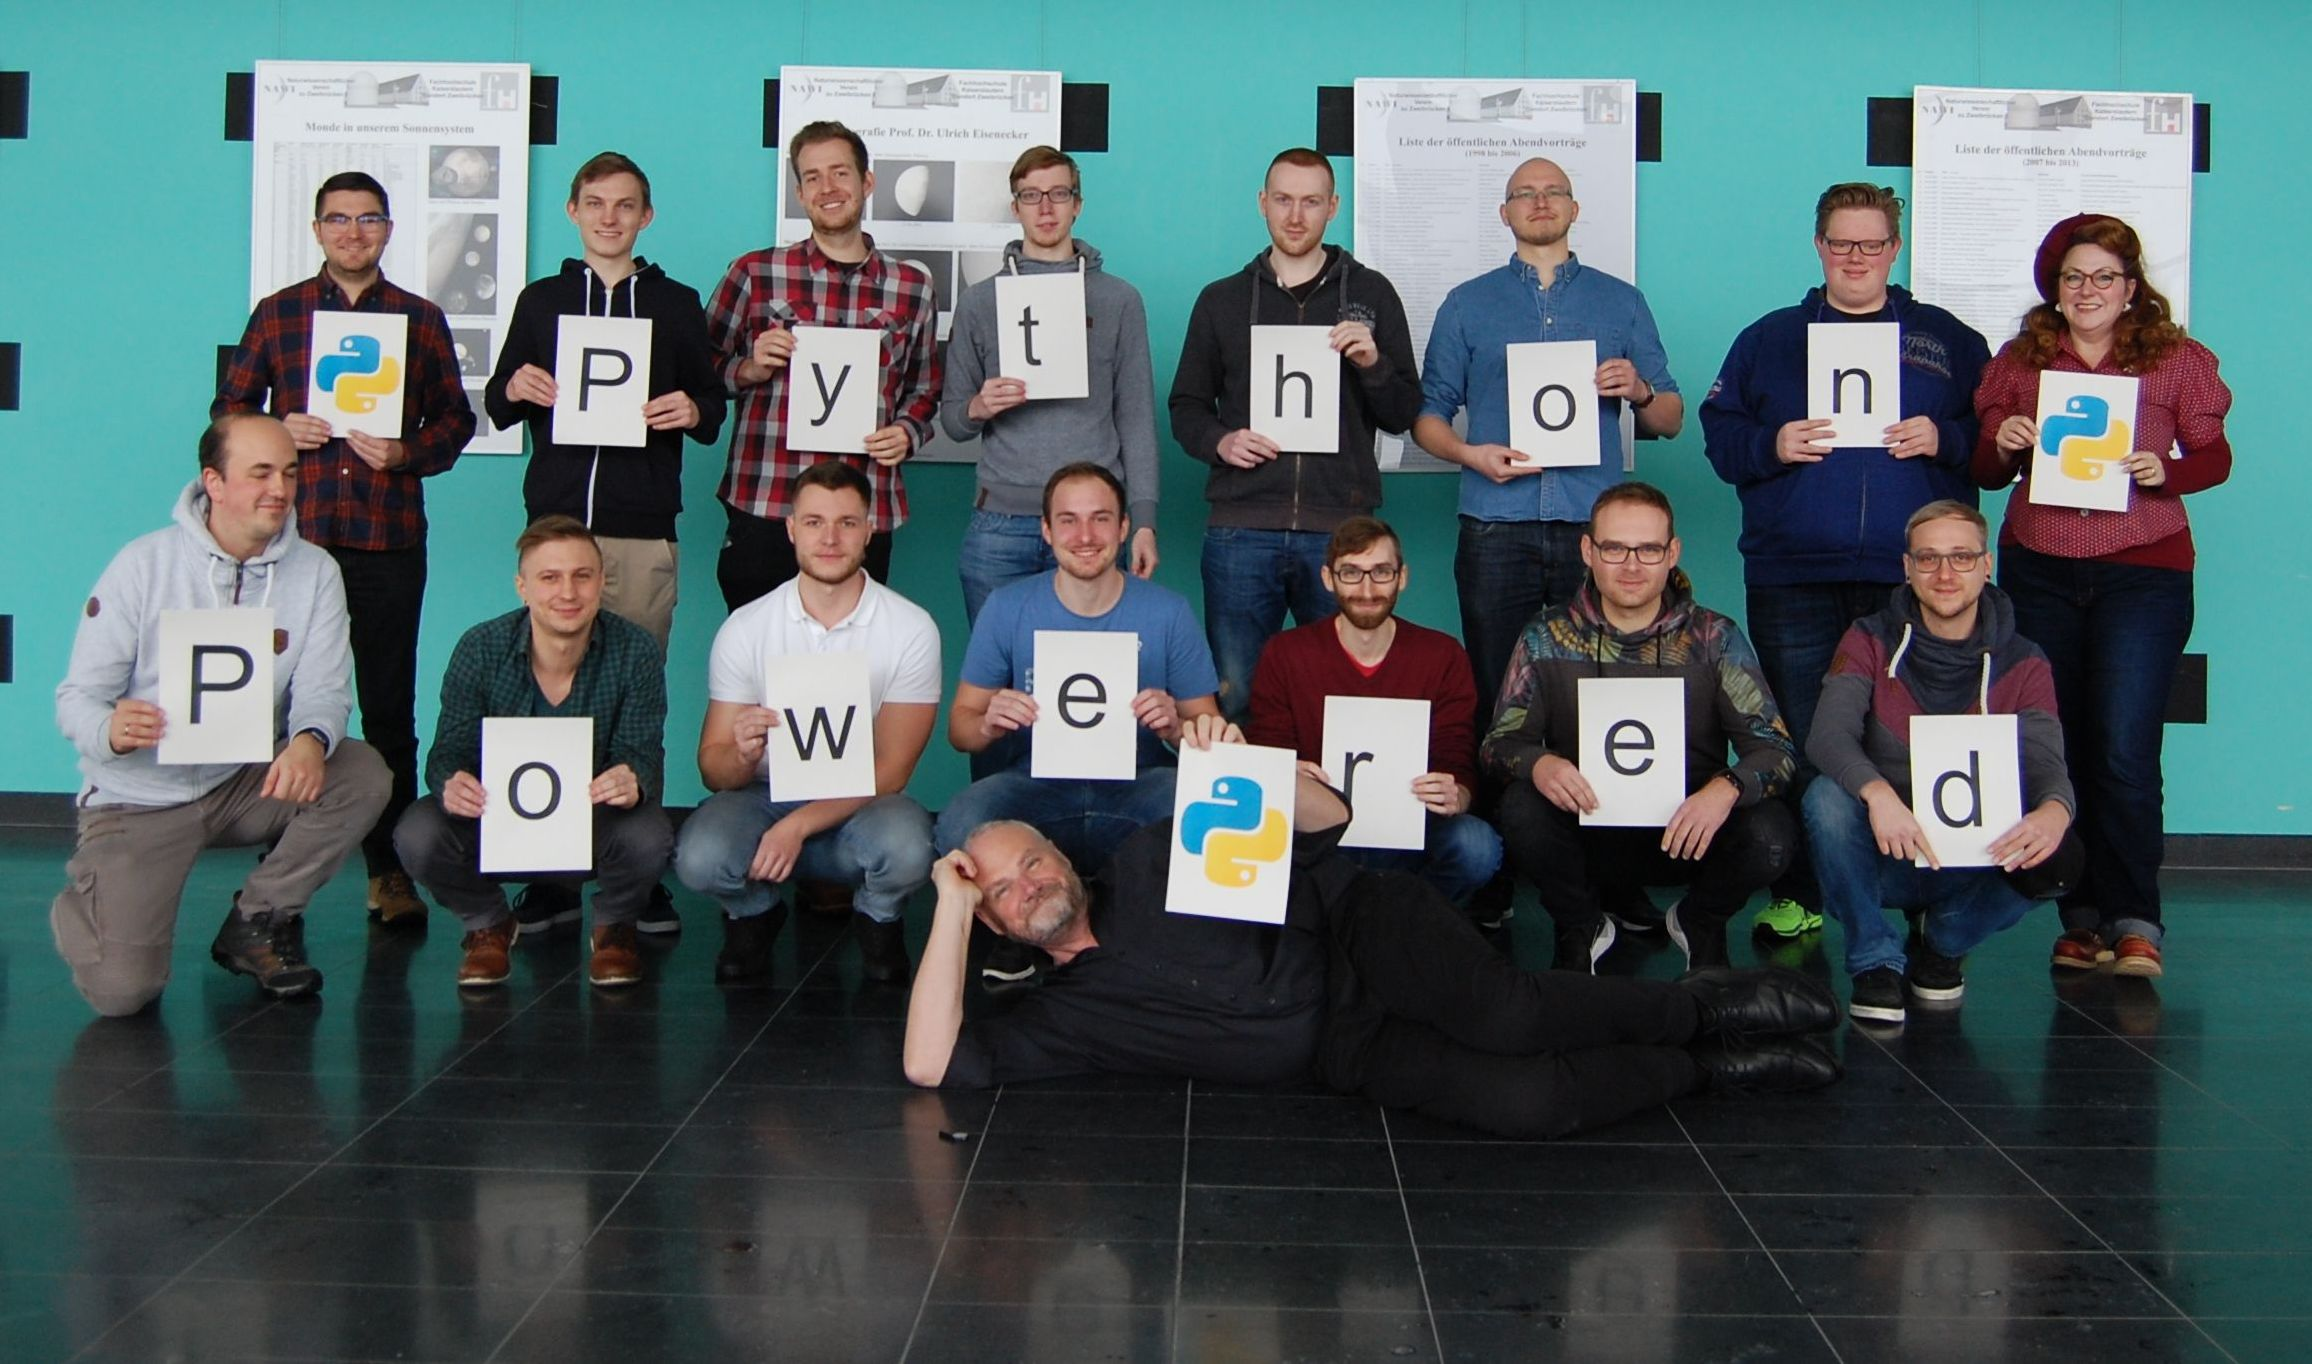
\includegraphics[width=\textwidth]{images/authors/theTeam}% Rotieren mit rotate=90
%\caption{\label{vorwort:team}Das Projektteam}
\end{figure}
\begin{tabular}{ll}
\centering
&Das Projektteam nach dem letzten Sprint Meeting\\
& im Januar 2019 von links nach rechts:\\
Hintere Reihe&Fabian Kalweit, Matthias Haselmaier, Marc Zintel,\\
                   &Robin Guth, Anatoli Sch�fer, Denis Schlusche,\\
                   &Kevin Konrad, Miriam Lohm�ller \\
Vordere Reihe&Mathias Fedder, Rainer Haffner, Lukas Kuhn,\\
                   &Sebastian Morsch, Julian Bernhart, Phillip Lauer,\\
                   &Christoph Seibel\\
Ganz vorne&Manfred Brill
\end{tabular}

\pagebreak
\subsection*{Die studentischen Autoren}
\begin{center}
\begin{tabular}{p{5cm}|l}
Julian  Bernhart&
\includegraphics[width=3cm]{images/authors/bernhart}\\
Eric Brunk&
\includegraphics[width=3cm]{images/authors/brunk}\\
Mathias Fedder&
\includegraphics[width=3cm]{images/authors/fedder}\\
Christopher Gross&\\
Robin Guth&\\
Rainer Haffner&\includegraphics[width=3cm]{images/authors/haffner}\\
Matthias Haselmaier&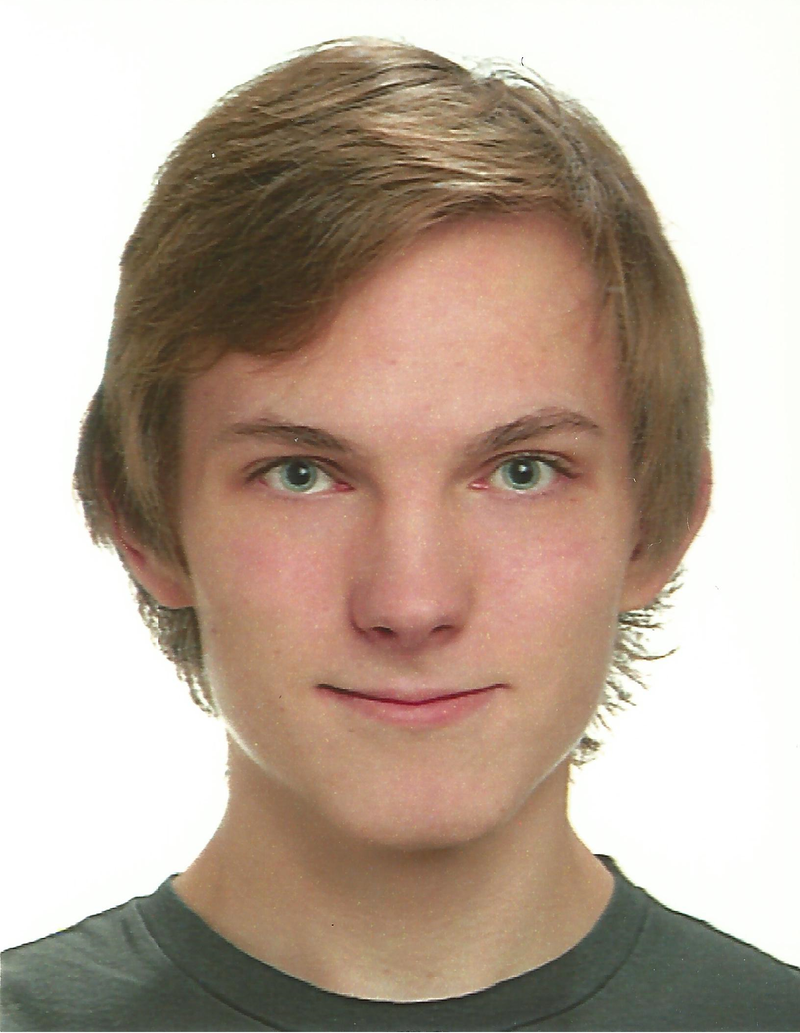
\includegraphics[width=3cm]{images/authors/haselmaier}\\
Kevin Konrad&\\
Lukas Kuhn&
\end{tabular}
\end{center}
\pagebreak
\begin{center}
\begin{tabular}{p{5cm}|l}
Philipp Lauer&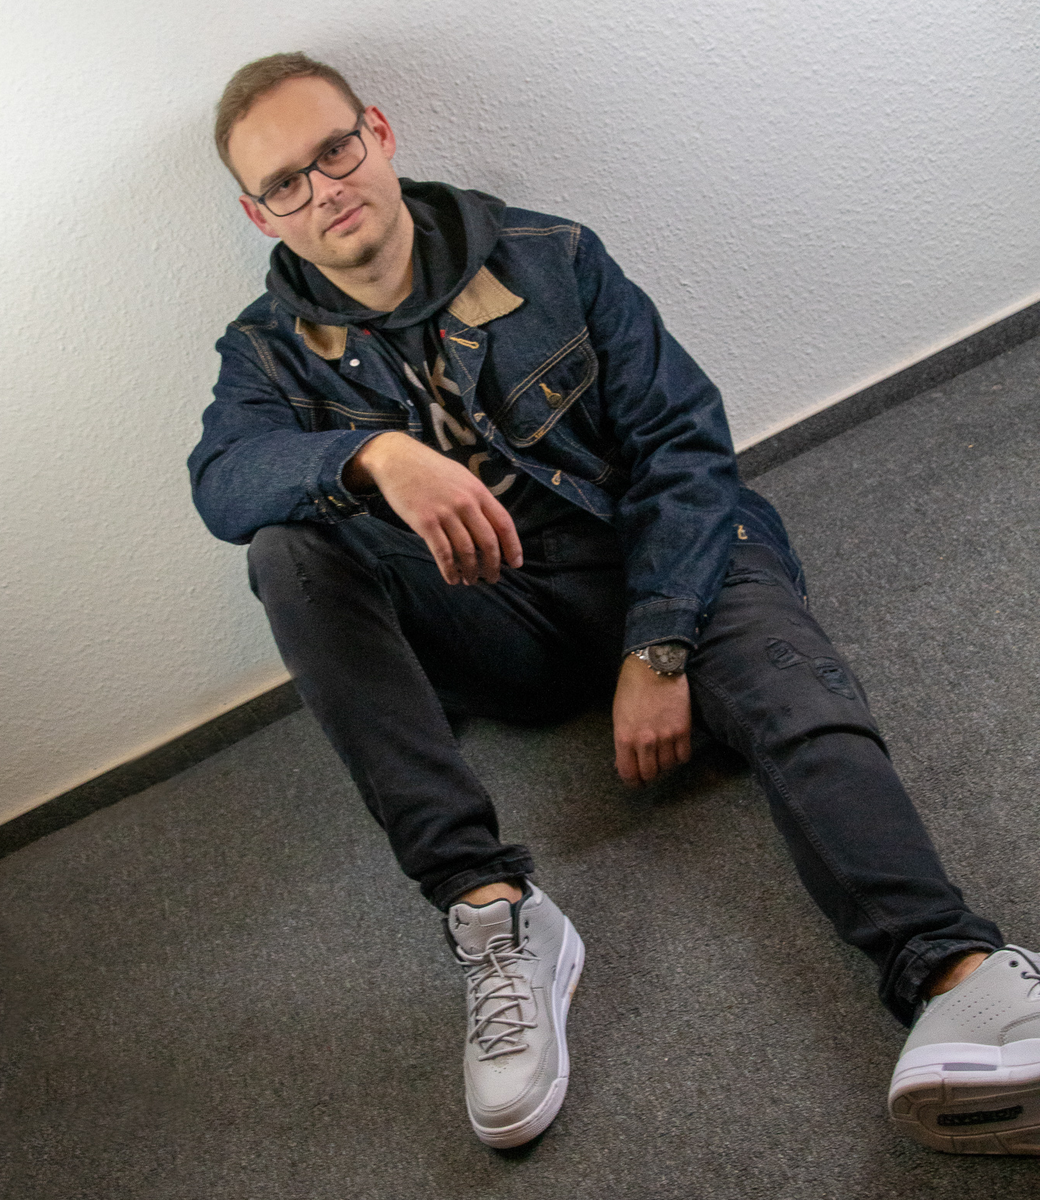
\includegraphics[width=3cm]{images/authors/lauer}\\
Sebastian Morsch&\\
Anatoli Sch�fer&\\
Denis Schlusche&\\
Christoph Seibel&
\includegraphics[width=3cm]{images/authors/seibel}\\
Marc Zintel&
\includegraphics[width=3cm]{images/authors/zintel}
\end{tabular}
\end{center} 
%
% Inhaltsverzeichnis
%
\tableofcontents
\clearevenpage
\pagenumbering{arabic}
%
%
%

% !TeX root = ../pythonTutorial.tex
\chapter{Grundlagen}

% !TeX root = ../../pythonTutorial.tex
\section{Was ist Python?}
\label{grundlagen:sec:WasIstPython}
Die Programmiersprache Python wurde Anfang der 1990er Jahre von Guido van Rossum als Universalprogrammiersprache entwickelt.
Der Name der Sprache beruht auf der Komikergruppe Monty Python.
Hierzu lassen sich auch zahlreiche Anspielung in der Dokumentation von Python finden.
Python wurde mit dem Ziel entworfen, eine einfache, gut verst�ndliche und �bersichtliche Programmiersprache zur Verf�gung zu stellen.
Dies soll nicht nur durch eine �bersichtliche Standardbibliothek erreicht werden, sondern auch durch die Modulare Erweiterbarkeit.
Im Folgenden wird die Programmiersprache Python in der Version 3 behandelt.

\section{Installation}

\label{grundlagen:sec:Installation}
Python \randnotiz{Installation} kann auf der Webseite \url{https://www.python.org} f�r eine Vielzahl von Betriebssystemen bezogen werden. 
Es stehen 32- und 64-Bit Versionen zur Verf�gung. 
Nach dem Start des Installationsassistenten wird der Nutzer durch die Installation gef�hrt. 
Der Ablauf der Installation unterscheidet sich je nach Betriebssystemen nur gering bis gar nicht.
Nach erfolgreichem Abschluss stehen dem Anwender verschiedene Programme f�r die Arbeit mit Python zur Verf�gung.
Im vom Nutzer gew�hlten Installationsverzeichnis befinden sich nun folgende Programme: 
\begin{description}
	\item[\textit{IDLE}] Standard IDE\footnote{Integrated Development Environment} f�r Python
	\item[\textit{Python}] Standard Konsolen Interpreter
	\item[\textit{Pythonw}] Standard Interpreter ohne Konsolenausgabe
\end{description}
Diese Programme reichen aus, um Code mit Python zu entwickeln. 
Der Python Interpreter kann in der Konsole mit dem Befehl \lstinline{python} aufgerufen werden. 
Die folgenden Abschnitte beschreiben Besonderheiten bei der Installation auf einzelnen Betriebssystemen. 
\subsection{Hinweis zur Installation unter Windows}
\label{grundlagen:sec:InstallationWindows}
Windows Nutzer m�ssen die Systemvariable f�r Python im Installationsassistenten hinzuf�gen lassen. 
Andernfalls kann Python nur im Installationsverzeichnis bzw. durch die Angabe des kompletten Pfads aufgerufen werden. 
In Abbildung \ref{grundlagen:img:InstallationWindows} ist die notwendige Auswahl zu sehen. 
\begin{figure}[ht]
	\centering
	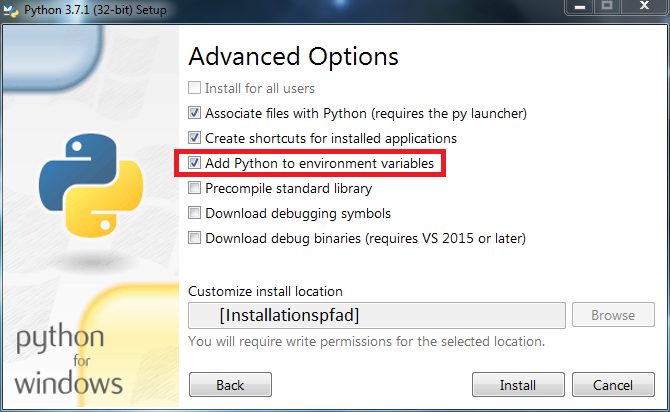
\includegraphics[scale=0.5]{images/InstallationWindows.png}
	\caption{Start des Installationsassistenten}
	\label{grundlagen:img:InstallationWindows}
\end{figure}
%
\subsection{Hinweis zur Installation unter Mac}
\label{grundlagen:sec:InstallationMac}
Im Folgenden wird die Installation unter macOS X gezeigt.

\begin{figure}[ht]
	\centering
	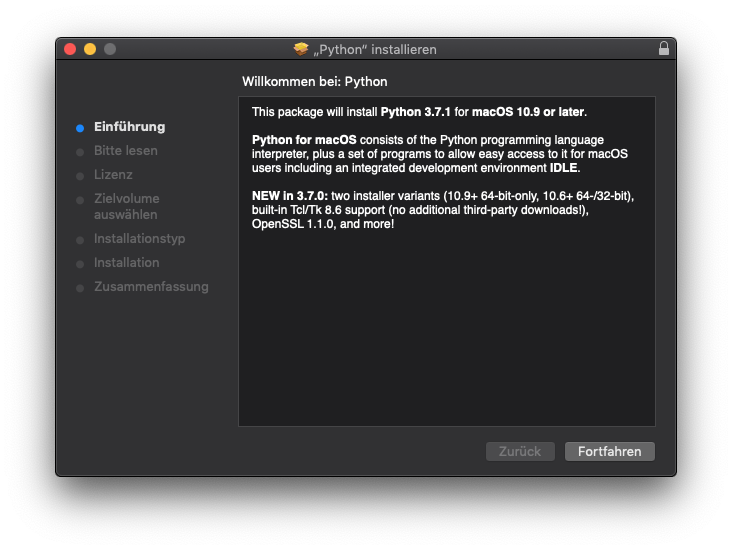
\includegraphics[scale=0.5]{images/InstallationMac.png} 
	\caption{Start des Installationsassistenten}
	\label{grundlagen:img:InstallationMac}
\end{figure}
Nach Ende der Installation befindet sich der Python Ordner im Finder (Dateiexplorer).

\begin{figure}[ht]
	\centering
	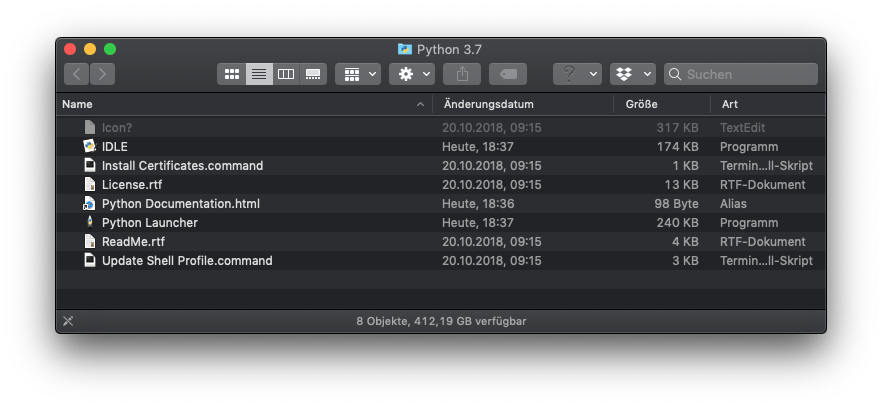
\includegraphics[scale=0.5]{images/PythonFinder.png} 
	\caption{Fertige Installation}
	\label{grundlagen:img:FinishInstall}
\end{figure}
Zuletzt wurde durch den Assistent unter \texttt{/Library/Frameworks/\\Python.framework} noch das Python Framework abgelegt.
Ohne das w�re die Arbeit mit Python unter Mac nicht m�glich.

\subsection{Hinweis zur Installation unter Linux(Ubuntu)}
\label{grundlagen:sec:InstallationLinux}
In diesem Kapitel wird die Installation f�r Ubuntu Version 18.04.1 LTS erl�utert.
Im Gegensatz zu den anderen Betriebssystemen, wird hier nur der Python Interpreter in der Version 3.6.6 mitgeliefert
Standard Entwicklungsumgebung IDLE ist nicht vorinstalliert.
Diese kann �ber das Paket IDLE nachtr�glich installiert werden.
Sollte die Arbeit mit Python noch nicht m�glich sein, kann durch den folgenden Befehl die Installation manuell angesto�en werden.

\begin{lstlisting}[language=BASH, label={grundlagen:lst:InstallationLinux}]
sudo apt-get install python3 python-doc
\end{lstlisting}

Diese Installation umfasst unter anderem auch die Dokumentation von Python.
Nach Abschluss der Installationsroutine kann wie mit jedem anderen Betriebssystem mit Python gearbeitet werden.

\section{Python Interpreter} 
\label{grundlagen:sec:Interpreter}
Die einfachste M�glichkeit, Python Code auszuf�hren, ist die direkte �bergabe des Codes an den sogenannten Python Interpreter. 
Dabei handelt es sich um eine Konsolenanwendung, die Code ausf�hren und gegebenenfalls auftretende Ergebnisse ausgeben kann. 
Dabei kann ein Nutzer den Code entweder direkt in die Konsole eingeben oder aus einer Datei auslesen lassen. 
Wie bei anderen Programmiersprachen auch, stehen f�r Python verschiedene IDEs zur Verf�gung, welche in Kapitel \ref{ides:section:ides} behandelt werden. 
F�r die ersten Versuche mit Python reicht der Interpreter jedoch v�llig aus. Dieser wird standardm��ig mit Python installiert.

In Abbildung \ref{grundlagen:img:Interpreter} ist der Interpreter zu sehen. 
Zus�tzlich zur Version werden auch noch der Herausgeber von Python sowie die Uhrzeit angezeigt.
Bereits jetzt kann erster Code ausgef�hrt werden.
Im Folgenden werden zu einzelnen Bestandteilen von Python Beispiele beigef�gt, die leicht im Interpreter ausf�hrbar sind. 
Es wird dem Leser empfohlen, sie zum besseren Verst�ndnis nachzuvollziehen, falls m�glich durch selbst�ndiges Ausprobieren.

\begin{figure}[ht]
	\centering
	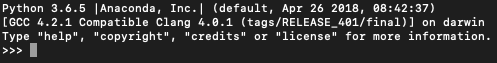
\includegraphics[width=0.8\textwidth]{images/Interpreter.png} 
	\caption{Ansicht nach Start des Interpreters}
	\label{grundlagen:img:Interpreter}
\end{figure}

\subsection*{Interaktiver Modus} 
\label{grundlagen:sec:InteraktiverModus}
Wird der Interpreter ohne Angabe einer Quellcodedatei gestartet, befindet dieser sich im interaktiven Modus. 
Der Nutzer kann hier direkt Anweisungen eingeben. Durch die Ausgabe der Zeichen $>>>$ zeigt die Konsole an, dass sie eine Anweisung erwartet. 
In Python existieren auch mehrzeilige Anweisungen. 
Nach der Eingabe der ersten Zeile werden die Zeichen $...$ ausgegeben, was bedeutet, dass Folgeanweisungen erwartet werden. 
\subsection*{Einlesen einer Datei}
\label{grundlagen:sec:EinlesenDatei}
Auf Dauer ist die direkte �bergabe des Codes an den Interpreter sehr unpraktisch. 
Um Code erneut nutzen zu k�nnen und zu speichern, kann dieser in Dateien abgelegt werden.
Dies kann mit einem simplen Texteditor erfolgen.
Dateien, die Python Code enthalten, werden mit der Dateiendung ''.py'' gekennzeichnet. 
Sie k�nnen direkt mit dem der Konsole ausgef�hrt werden.
Dazu muss Python der relative Pfad der Pythondatei (.py-Endung) �bergeben werden.  
\begin{lstlisting}[language=BASH, label={grundlagen:lst:BashStartPython1}]
python <Relativer Dateipfad der Pythondatei>
\end{lstlisting} 
Da nur der relative Pfad angegeben werden muss, muss lediglich der Dateiname angegeben werden, falls die Konsole sich bereits im selben Verzeichnis wie die zu �ffnende Datei befindet.
\section{Syntax}
\label{grundlagen:sec:Syntax}
Im \randnotiz{Syntax} Folgenden werden wichtige Grundkonzepte der Programmiersprache\\ \mbox{Python} erl�utert.
%Benoetigt um korrekten Zeilenumbruch zu erzwingen
\subsection{Allgemeine Strukturen}
\label{grundlagen:sec:AllgemeineStrukturen}
Anders als bei anderen Programmiersprachen wie beispielsweise Java oder C++, ben�tigt Python keine Klassenkonstrukte oder main-Methoden zur Ausf�hrung. 
Das bedeutet, dass einzelne Anweisungen in Python korrekt ausgef�hrt werden k�nnen. 
Sollten f�r die Bearbeitung von komplexeren Problemen objektorientierte Ans�tze ben�tigt werden, kann auch dies mit Python umgesetzt werden. 
Weitere Informationen zur Objektorientierung mit Python finden sich im weiteren Verlauf des Python Tutorials.
F�r den Moment reicht es f�r den Leser zu wissen, dass Anweisungen bereits zeilenweise ausgef�hrt werden k�nnen. 
Das kann sehr simpel getestet werden, indem der Python Interpreter als einfacher Taschenrechner genutzt wird. 
In Abbildung \ref{grundlagen:img:AusdrueckeInInterpreter} wird dies gezeigt. Einfache Ausdr�cke wie Summen, Subtraktionen, Multiplikationen und Divisionen k�nnen direkt eingegeben werden. 
Nach Bet�tigung der Eingabe-Taste liefert Python das Ergebnis des Ausdrucks.\\
\begin{figure}
	\centering
	\includegraphics[width=1\textwidth]{images/AusdrueckeInInterpreter.png} 
	\caption{Einfache Ausdr�cke im Python Interpreter}
	\label{grundlagen:img:AusdrueckeInInterpreter}
\end{figure}
\subsection{Leerzeichen und Einr�ckung}
\label{grundlagen:sec:LeerzeichenEinrueckung}
Um in Python Bl�cke auszuzeichnen, werden im Gegensatz zu Java oder C++ keine geschweiften Klammern genutzt.
In Python werden Bl�cke durch das Einr�cken der Zeilen markiert. 
Hierf�r sind entweder der Tabulator oder vier aufeinander folgende Leerzeichen vorgesehen.
\subsection{Kommentare}
\label{grundlagen:sec:Kommentare}
Innerhalb der Programmiersprache Python wird zwischen Zeilen- und Blockkommentaren unterschieden.
Zeilenweise Kommentare werden durch das Rautensymbol \lstinline$\#$ eingeleitet.
Blockkommentare hingegen werden durch drei aufeinander folgende Anf�hrungszeichen \lstinline$"""$ jeweils zu Beginn und am Ende des Kommentars markiert.
Hier wird jeweils ein Beispiel gezeigt:

\lstinputlisting[language=Python,label={grundlagen:lst:Kommentare}]{chapters/basics/src/comment.py}
\subsection{Typsicherheit}
\label{grundlagen:sec:Typsicherheit}
Anders als bei Java und C++ ist Python eine nur schwach typisierte Sprache.
Somit ist bei der Initialisierung keine Typangabe erforderlich.
Der Datentyp wird beim Initialisieren dynamisch ermittelt und automatisch zugewiesen.
Um einer Variable trotzdem einen gew�nschten Typ zuzuweisen, kann man sie einfach mit dem entsprechenden Typ initialisieren.
Weitere Informationen zu Datentypen werden in Abschnitt \ref{basicdatatypes:sec:ElementareDatentypen} erl�utert.
\section{Beispiel \glqq Hello World!\grqq}
\label{grundlagen:sec:HalloWorld}
Einfache \randnotiz{Beispiel} Ausgaben k�nnen mit der print()- Anweisung gemacht werden. 
Innerhalb der Klammern muss ein String �bergeben werden, sprich eine einfache Zeichenkette. 
Diese wird durch umschlie�ende einfache oder doppelte Anf�hrungszeichen markiert (''EinString''/'EinString'). 
Der Einfachheit halber, wird hier noch auf die genaue Erkl�rung der einzelnen Bestandteile der Anweisung verzichtet. 
Ein einfaches ''Hello-World!''-Programm ben�tigt in Python nur eine Zeile: 
\lstinputlisting[language=python, label={grundlagen:lst:HalloWorld}]{chapters/basics/src/helloworld.py} 
Es handelt sich dabei um ein vollst�ndiges Python-Programm, das in dieser Form ausgef�hrt werden kann. 
Wie bereits erl�utert, werden anders als bei Java oder C++ keine Klassenkonstrukte oder main-Methoden ben�tigt.

%\uebung
%\aufgabe{grundlagen01} 
%\aufgabe{grundlagen02}

\uebungTutorial{grundlagen01}{grundlagen02}


% !TeX root = ../../pythonTutorial.tex


\section{IDEs}

Python Programmierung mit der IDLE (in Python integrierte Entwicklungsumgebung) oder Python Shell sind gute M�glichkeiten um den Einstieg in Python  zu vereinfachen. Ein grunds�tzliches Verst�ndnis der Sprache und erste kleine Programme lassen sich so bew�ltigen. Sobald jedoch gr��ere Programme oder Projekte anstehen kann es mit diesen Tools schnell frustrierend werden.

Eine passende IDE (Integrierte Entwicklungsumgebung) oder selbst ein einfacher Code-Editor kann einem das leben deutlich vereinfachen. Im folgenden werden einige geeigneten IDEs f�r Python vorgestellt und f�r jede einige Vor- und Nachteile aufgezeigt.

\textbf{Was ist eine IDE?}

Integrierte Entwicklungsumgebungen vereinen wichtige Tools f�r das Erstellen von Software unter einer Oberfl�che. Dazu z�hlen Editor mit Syntaxhervorhebung, Compiler, Debugger, Interpreter und weitere Werkzeuge, die dem Entwickler die Arbeit erleichtern.

Durch den Austausch zwischen Werkzeugen innerhalb der IDE k�nnen Arbeitsg�nge erleichtert und beschleunigt werden. Fehler im Quelltext beispielsweise k�nnen direkt in der entsprechenden Zeile markiert werden.

\textbf{Anforderungen an eine geeignete Python Entwicklungsumgebung}

Es gibt ein paar Grundanforderungen an eine geeignete oder gute Python Entwicklungsumgebung:

\begin{description}
\item[Debugging Unterst�tzung]\hfill \\
Schrittweise durch den Code zu wandern, w�hrend dieser ausgef�hrt wird, ist eine weiter Grundaufgabe einer IDE.
\item[Syntax Highlighting]\hfill \\
Farbliche Markierungen erleichtern die Suche nach bestimmten Keywords. Die Lesbarkeit des Codes wird hierdurch verbessert.
\item[Automatische Codeformatierung]\hfill \\
Eine gute IDE erkennt das Zeilenende beispielsweise nach einem \textit{While-Statement} und r�ckt die n�chste Zeile automatisch ein.
\item[Ausf�hren des Codes innerhalb der IDE]\hfill \\
Wenn der Code au�erhalb der IDE ausgef�hrt werden muss, ist es eher ein Text-Editor als eine IDE.
\item[Interaktive Console]\hfill \\
Live Ein- und Ausgabe einzelner Codezeilen.
\item[Fehlererkennung]\hfill \\
Syntaxfehler sollten automatisch markiert werden und Runtime-Fehler genannt werden.
\end{description}

\subsection{Einige IDEs vorgestellt}
\textbf{Eclipse} \\
Wer schon mit Java programmiert hat, ist wohl schon mal auf Eclipse gesto�en. Durch die Installation von PyDeth l�sst sich Eclipse gut (und kostenlos) f�r die Python-Entwicklung erweitern und bietet dabei wichtige Features, wie zum Beispiel Code Completion, Python Debugging, eine interaktive Python Konsole oder das Einbinden von Django.

\textbf{Vorteile:}
Wenn Eclipse bereits auf dem Rechner vorhanden ist, gen�gt der Download der PyDeth Erweiterung, welche nach einem Neustart von Eclipse sofort eingebunden ist.

\textbf{Nachteile:}
Der Einstieg in die Python Programmierung f�r Eclipse-Neulinge kann in der sehr gro�en Entwicklungsumgebung Eclipse zu Schwierigkeiten f�hren.

\textbf{Visual Studio} \\
Die IDE aus dem Hause Microsoft bietet viele eigene Erweiterungen und Entwicklungs-Features an, welche dem Entwickler eine gute Individualisierungsm�glichkeit bieten. Die Visual Studio Python Tools erm�glichen es, alle �blichen Entwicklungsm�glichkeiten bei Programmierung mit Python zu nutzen. Visual Studio ist sowohl in der Community-Version umsonst, aber auch in einem Bezahlmodell verf�gbar.

Visual Studio Community kann kostenlos �ber folgenden Link heruntergeladen werden: https://visualstudio.microsoft.com/de/vs/community/

\textbf{Nachteile:}
Der Download ausschlie�lich f�r die Python-Programmierung ist recht gro� (3-4GB). Es m�ssen sowohl das Programm an sich, als auch die Python-Erweiterung heruntergeladen werden. Visual Studio ist ausschlie�lich f�r Windows und MacOs verf�gbar. Eine Linux-Variante wird allerdings von Visual Studio Code angeboten. Vergleichbar mit Eclipse ist auch Visual Studio nicht sonderlich einsteigerfreundlich.

\textbf{Atom}  \\
Etwas schlichter geht es im Atom Editor zu. Das klare und strukturierte Interface ist auch f�r Einsteiger gut verst�ndlich und dient daher als geringere H�rde, die ein Neuling �berwinden muss, als die �berladenen Interfaces von Eclipse oder Visual Studio. Python kann durch eine Erweiterung nachtr�glich installiert werden, welche w�hrend der Laufzeit hinzugef�gt werden kann.

\textbf{Vorteile:}
Einsteigerfreundliche Alternative mit geringem Download- und Installationsumfang, sowie Plattformunabh�ngigkeit.

\textbf{Nachteile:}
\textit{Build-} und \textit{Debugging-Support} sind keine eingebauten Features, sondern nur als Community-Addon verf�gbar.


\textbf{PyCharm} \\
PyCharm ist (wie es der Name vermuten l�sst) eine IDE explizit f�r Python. Es ist neben der Hauptdatei keine Erweiterung n�tig, ein neues Projekt kann sofort gestartet und mit dem Programmieren sofort begonnen werden. PyCharm ist Plattformunabh�ngig und sowohl in einer freien Open-Source-Version nutzbar, als auch in einer kostenpflichtigen Pro-Version erh�ltlich.

\textbf{Vorteile:}
PyCharm bietet einen vielf�ltigen Support an und eine sehr aktive Community. Egal an welcher Stelle man ein Problem hat, es wird einem mit gro�er Wahrscheinlichkeit geholfen.  

\textbf{Nachteile:}
Die Ladezeiten sind vergleichbar lang und an manchen Stellen finden sich kleinere Usability-Schwachpunkte.


% !TeX root = ../../pythonTutorial.tex

\section{Elementare Datentypen}
\label{basicdatatypes:sec:ElementareDatentypen}

�hnlich wie bei Java und C oder C++ gibt es auch in Python Variablen. Allerdings gibt es dabei immense Unterschiede zu den anderen Programmiersprachen, weshalb sich ein genauerer Blick auf die einzelnen Datentypen in jedem Fall lohnt. Bei vielen bekannten Sprachen wird einer Variablen ein bestimmter Datentyp zugeordnet (deklariert). Der Datentyp kann darauf folgend zur Laufzeit nicht wieder ge�ndert werden, der Wert innerhalb des Datentyps allerdings schon. So lassen sich in eine Variable des Typ Integer beispielsweise keine String-Werte speichern. In Python hingegen ist dies ohne weiteres m�glich. Hier wird g�nzlich auf eine explizite Typdeklaration verzichtet. Zeigt eine Variable beispielsweise auf eine ganze Zahl, so wird diese als ein Objekt vom Typ Integer interpretiert. Allerdings ist es m�glich, diese im n�chsten Schritt einfach auf ein String-Objekt zeigen zu lassen. Dies ist in Python m�glich, weil eine Variable ein Objekt lediglich referenziert und dadurch keinem Typ zugewiesen wird.\\
Betrachten wir nun die Datentypen etwas genauer.

\subsection{Zahlenoperatoren}
\label{basicdatatypes:sec:Zahlenoperatoren}

Da in Python auf Typdeklaration verzichtet wird, muss dies beim Anlegen von Variablen nicht ber�cksichtigt werden. Wird eine ganze Zahl (Integer) ben�tigt, kann diese, falls n�tig, auch in eine Gleitkommazahl (float) umgewandelt werden, ohne viel am Code zu �ndern. Python deklariert im Hintergrund selbst und spart so unn�tige Komplexit�ten und Fehlerquellen. (Beispiel \ref{refzahl})

\begin{lstlisting}[label=refzahl]
# Zahlenoperatoren
i = 42
type(i)
// Ausgabe: <class 'int'>
i = 42.22
type(i)
// Ausgabe: <class 'float'>
\end{lstlisting}

\textbf{Boolean}

Boolean gibt an, ob ein Statement \textit{true} oder \textit{false} ist. Dadurch lassen sich Fallunterscheidungen oder Abfragen erm�glichen. (Beispiel in Listing \ref{basicDatatypes:lst:refbool})

\begin{lstlisting}[label=basicDatatypes:lst:refbool]
# Boolean
i = True
i
// Ausgabe: True

\end{lstlisting}

\textbf{String}

Der String ist eine Zeichenkette, also eine Aneinanderreihung von verschiedenen Zeichen. Dazu z�hlen W�rter, aber auch beispielsweise Hexadezimal-Codes oder E-Mail Adressen.

Wie in den meisten objektorientierten Programmiersprachen lassen sich auch in Python die einzelnen Zeichen eines Strings abrufen, indem der dazugeh�rige Index abgefragt wird.

Wie in Listing \ref{basicDatatypes:lst:refstring} kann die L�nge des gesamten Strings durch einfache Abfrage angezeigt werden.

\begin{lstlisting}[label=basicDatatypes:lst:refstring]
# Strings
i = "Python"
print (i)
// Ausgabe: Python

print(i[0])
// Ausgabe: P

print(len(i))
// Ausgabe: 6

\end{lstlisting}

\subsection{ENUMs}
\label{basicdatatypes:sec:Enums}

Enums dienen in den objektorientierten Programmiersprachen zur Aufz�hlung von Ausdr�cken einer endlichen Menge. So werden zum Beispiel Jahreszeiten, Monate oder Farben oft als Enums umgesetzt (vgl. Listing \ref{refenum}).


\begin{lstlisting}[label=refenum]
# Enums
from enum import Enum
class Color(Enum):
    RED = 1
    GREEN = 2
    BLUE = 3

\end{lstlisting}

\subsection{NULL oder NONE}
\label{basicdatatypes:sec:NullNone}
Das Schl�sselwort \textit{NULL} wird in vielen Programmiersprachen genutzt. Die Idee dahinter ist einer Variable ein neutrales Verhalten zu geben. Das �quivalent zu \textit{NULL} in Python ist \textit{NONE}. Der Vorteil ist, dass \textit{NONE} exakt der Aufgabe des Schl�sselworts entspricht. Ein Anwendungsfall f�r \textit{NONE} w�re beispielsweise um zu �berpr�fen, ob die Verbindung zu einer Datenbank aufgebaut werden konnte oder nicht (Siehe Beispiel \ref{refnone}).

\begin{lstlisting}[label=refnone]
# NULL oder NONE
database_connection = None

try:
    database = MyDatabase(host, user, password, database)
    database_connection = database.connect()
except DatabaseException:
    pass

if database_connection is None:
// Solange die Variable "NONE", keine Verbindung aufgebaut
    print('The database could not connect')
else:
    print('The database could connect')

\end{lstlisting}

\subsection{Referenz, Identit�t und Kopie}
\label{basicdatatypes:sec:Referenzen}

Wie bereits erw�hnt wurde, wird in Python eine Variable keinem Typ zugewiesen. Zeigt eine Variable jedoch st�ndig auf ein neues Objekt, sind Verwechslungen innerhalb des Codes m�glich. Um dies zu vermeiden bietet sich die Identit�tsfunktion id() an. Diese hilft uns dabei, die verschiedenen Instanzen voneinander zu unterscheiden. Jede Instanz hat dabei unabh�ngig von ihrem Wert und ihrem Typ eine eindeutige Identit�t. \\

Dies ist in Python m�glich, weil eine Variable ein Objekt lediglich referenziert und dadurch keinem Typ zugewiesen wird.

\uebung
\aufgabe{DatatypesAufgabe1}

%\uebungTutorial{DatatypesAufgabe1} 


% !TeX root = ../../pythonTutorial.tex

\section{Kontrollstrukturen}

Die Kontrollstrukturen in Python haben einen formalen Unterschied zu Java oder C++, funktional allerdings sind sie identisch. In Python werden keine geschweiften Klammern genutzt, um die Bl�cke der einzelnen Abfragen abzugrenzen. Dazu gen�gt das Einr�cken der Anweisung. Dies gilt sowohl f�r Bedingungen und Conditional Expressions, als auch f�r Schleifen. Im Folgenden schauen wir uns die einzelnen Strukturen im Detail und mit Beispielen an.

\subsection{If-then-else}

Die if-then-else-Struktur erm�glicht es, wie wir es bereits kennen, simple wenn-dann Abfragen zu t�tigen.\\
Mehrere Abfragem�glichkeiten werden mit elif markiert. Vergleich hierzu Listing \ref{kontrollstrukturen:lst:refif}.



\begin{lstlisting}[label=kontrollstrukturen:lst:refif]
# If-then-else
if statement1:
	print("Fall 1")
elif statement2:
	print("Fall 2")
else:
	print("Fall 3")
\end{lstlisting}

\textbf{Conditional Expressions}

Die Conditional Expressions (engl. bedingte Ausdr�cke) stellen eine kompaktere Schreibweise als if-then-else-Bedinungen dar. Ein Beispiel ist in Listing \ref{kontrollstrukturen:lst:refcond} zu finden. 

\begin{lstlisting}[label=kontrollstrukturen:lst:refcond]
# Conditional Expressions
# Klassisches If-Else
if wort == "start":
	x = "los"
else:
	x = halt"
	
# If-Else als Conditional Expression
x = ("los" if wort == "start" else "halt")

\end{lstlisting}


\subsection{Schleifen}

Python hat sowohl bedingte, als auch Z�hler-Schleifen, welche wir uns beide im Folgenden genauer ansehen werden (vgl. Listing \ref{kontrollstrukture:lst:refwhile} und \ref{kontrollstrukture:lst:reffor}). Schleifen bestehen aus einer Anweisung und einem Kontrollblock, welcher solange durchlaufen wird, bis die Anweisung oder ein Abbruchkriterium erf�llt wurde. Schleifen, die niemals ein Abbruchkriterium erf�llen und so endlos durchlaufen werden, hei�en Endlosschleifen. Diese f�hren dazu, dass der Interpreter irgendwann aufgibt und abbricht.

\begin{lstlisting}[label=kontrollstrukture:lst:refwhile]
# While-Schleife
while Bedingung:
	Anweisungsblock
	if Bedingung:
		Anweisungsblock
		continue
	if Bedingung:
		Anweisungsblock
		break
	Anweisungsblock

\end{lstlisting}

\begin{lstlisting}[label=kontrollstrukture:lst:reffor]
# While-Schleife
for Variable in Objekt:
	Anweisungsblock
	if Bedingung:
		Anweisungsblock
		continue
	Anweisungsblock
	if Bedingung:
		Anweisungsblock
		break
	Anweisungsblock

\end{lstlisting}



\subsection{Ausdr�cke und Operatoren}

Die meisten Operatoren f�r Zahlenwerte sind in Python �hnlich wie bei anderen Programmiersprachen. Im folgenden wird eine �bersicht gegeben.

\begin{table}[h]

\begin{tabular}{|p{0.15\textwidth}|p{0.5\textwidth}|p{0.25\textwidth}|}
\hline
\multicolumn{1}{|c|}{\textbf{Operator}} & \multicolumn{1}{c|}{\textbf{Bezeichnung}} & \multicolumn{1}{c|}{\textbf{Beispiel}} \\ \hline
\hline
+, - & Addition, Subtraktion & 4 - 3 \\ \hline
*, \% & Multiplikation, Rest & 24 \% 5 \newline Ergebnis: 4 \\ \hline
/ & Division & 10 / 3 \newline Ergebnis: 3.33333333333335 \\ \hline
// & Ganzzahldivision & 10 // 3 \newline Ergebnis: 3 \\ \hline
+x, -x & Vorzeichen & -5 \\ \hline
** & Exponentiation & 2 ** 4 \newline Ergebnis: 16 \\ \hline 
or, and, not & Boolsches Oder / Und / Nicht & (a or b) and c \\ \hline
in & Element von & 1 in [1,2,3]  \\ \hline
<, <=, >, >=, !=, == & Vergleichsoperatoren & 4 <= 5 \\ \hline
\end{tabular}
\caption{Ausdr�cke und  Operatoren}

\end{table}




% !TeX root = ../../pythonTutorial.tex
\section{Collections}
\label{collections:sec:collections}

In Python 3 existieren nativ die vier Datenstrukturen List, Tuple, Set und Dictionary, welche im Folgenden vorgestellt werden.

\subsection{List}
\label{collections:sec:list}
\randnotiz{List}

Die Datenstruktur List bietet einen geordneten und ver�nderbaren Beh�lter f�r Python-Objekte, der Duplikate von Elementen erlaubt. Da eine List immer sortiert ist, k�nnen einzelne Elemente aus der Datenstruktur �ber den entsprechenden Index ausgew�hlt und ver�ndert werden. Python unterst�tzt intern keine Arrays, alternativ hierzu kann eine List verwendet werden.

Eine List kann wie folgt initialisiert werden:
\lstinputlisting[language=Python]{chapters/basics/src/list/ListInit.py}
\label{collections:lst:listinit}

Dabei kann sie jegliche Art von Objekten beinhalten; der Datentyp spielt hierbei keine Rolle. 

Beispiel:
\lstinputlisting{chapters/basics/src/list/ListDataType.py}
\label{collections:lst:listdatatype}

Im Gegensatz zu Java und C++ muss der Programmierer darauf achten und sicherstellen, dass die Datenstruktur mit Werten des entsprechenden Datentyps bef�llt wird, um Fehler aufgrund unterschiedlicher Datentypen zu vermeiden.

Der Inhalt einer List kann �ber die \lstinline$print()$-Methode ausgegeben werden. Im folgenden Beispiel werden verschiedene Elemente der List auf der Konsole ausgegeben.
Wird die List als Parameter gew�hlt, wird der Inhalt ausgegeben.
\lstinputlisting{chapters/basics/src/list/ListPrint.py}
\label{collections:lst:listprint}

Wie zuvor erw�hnt, �hnelt die Verwaltung einer List der eines Arrays aus Java oder C++. Durch die Verwendung eines Index k�nnen einzelne Elemente ausgew�hlt oder ver�ndert werden.
\lstinputlisting{chapters/basics/src/list/ListIndex.py}
\label{collections:lst:listindex}

Python erlaubt die Nutzung von negativen Indizes. Mit diesen kann der Inhalt der List in umgekehrter Reihenfolge ausgegeben werden. Ein Index von \lstinline$-1$ wird dem letzten Element der List zugeordnet, \lstinline$-2$ dem vorletzten.
\lstinputlisting{chapters/basics/src/list/ListNegativeIndex.py}
\label{collections:lst:lsitnegativeindex}

In Python existiert f�r die Datenstruktur List keine Methode, die mit \\ \lstinline$contains()$ in Java oder der \lstinline$find()$ aus C++ vergleichbar ist. Stattdessen stehen die Membership Operatoren \lstinline$in$ oder \lstinline$not$ \lstinline$in$ zur Verf�gung, die auf eine beliebige Sequenz oder die hier beschriebenen Collections angewendet, Auskunft dar�ber gibt, ob das spezifizierte Element darin enthalten ist.
\lstinputlisting{chapters/basics/src/list/ListInOperator.py}
\label{collections:lst:listinoperator}
    
Der Python Interpreter stellt nativ einige Funktionen zur Verf�gung. Eine davon ist die \lstinline$len()$-Methode, die die Anzahl an Elementen in einem Objekt liefert.
\lstinputlisting{chapters/basics/src/list/ListLen.py}
\label{collections:lst:listlen}
    
Das \lstinline$del$-Statement erlaubt das L�schen einzelner Elemente oder der gesamten List.
\lstinputlisting{chapters/basics/src/list/ListDelete.py}
\label{collections:lst:listdel}
    

\subsubsection{Methoden einer List}
\label{collections:sec:listmethodes}
\randnotiz{List-Methoden}

\textbf{append():}
F�gt am Ende der List ein Objekt hinzu.
\lstinputlisting{chapters/basics/src/list/ListAppend.py}
\label{collections:lst:listappend}

\textbf{clear():}
Entfernt s�mtliche Objekte aus der List.
\lstinputlisting{chapters/basics/src/list/ListClear.py}
\label{collections:lst:listclear}

\textbf{copy():}
Liefert eine Kopie der List.
\lstinputlisting{chapters/basics/src/list/ListCopy.py}
\label{collections:lst:listcopy}
    
%\newpage
\textbf{count():}
Liefert die Anzahl des spezifizierten Objekts in der List.
\lstinputlisting{chapters/basics/src/list/ListCount.py}
\label{collections:lst:listcount}

\textbf{extend():} 
F�gt der \lstinline$liste1$ den Inhalt der \lstinline$liste2$ am Ende hinzu.
\lstinputlisting{chapters/basics/src/list/ListExtend.py}
\label{collections:lst:listextend}
    
\textbf{index():}
Liefert den Index der Position, an der sich das erste spezifizierte Objekt in der List befindet.
\lstinputlisting{chapters/basics/src/list/ListIndexMethode.py}
\label{collections:lst:listindexmethode}
    
\textbf{insert():}
F�gt ein Objekt an der gew�hlten Position der List hinzu.
\lstinputlisting{chapters/basics/src/list/ListInsert.py}
\label{collections:lst:listinsert}

\textbf{pop():}
Entfernt das Objekt, das sich an der durch den Index spezifizierten Position befindet.
\lstinputlisting{chapters/basics/src/list/ListPop.py}
\label{collections:lst:listpop}
    
\textbf{remove():}
Entfernt das erste Objekt der List, das der Spezifikation entspricht.
\lstinputlisting{chapters/basics/src/list/ListRemove.py}
\label{collections:lst:listremove}
    
\textbf{reverse():}
Invertiert die Folge der Objekte in der List.
\lstinputlisting{chapters/basics/src/list/ListReverse.py}
\label{collections:lst:listreverse}

\textbf{sort():}
Sortiert die List.
\lstinputlisting{chapters/basics/src/list/ListSort.py}
\label{collections:lst:listsort}

    
\subsection{Tuple}
\label{collections:sec:tuple}
\randnotiz{Tuple} 

Ein Tuple stellt einen geordneten und unver�nderbaren Beh�lter f�r Python-Objekte dar. Dieser erlaubt, wie eine List, Duplikate und den Zugriff auf einzelne Elemente �ber einen Index. Tuple sind Datenstrukturen, die ausschlie�lich gelesen werden k�nnen.

Ein Tuple wird mit folgender Syntax erzeugt:
\lstinputlisting{chapters/basics/src/tuple/TupleInit.py}
\label{collections:lst:tupleinit}

Es ist m�glich, leere Tuple zu erzeugen. Wie zuvor erw�hnt, ist deren Inhalt unver�nderlich.

\subsubsection{Arbeiten mit einem Tuple}
\label{collections:sec:workwithtuple} 

Der Inhalt eines Tuple kann, analog zur List, auf der Konsole ausgegeben werden. Das Zuweisen eines neuen Objekts mittels Index f�hrt im Gegensatz zur List zu einem Fehler.
\lstinputlisting{chapters/basics/src/tuple/TupleIndex.py}
\label{collections:lst:tupleindex}    
    
Die Verwendung der Operatoren \lstinline$in$ und \lstinline$not in$ ist, wie die \lstinline$len()$-Methode, analog zur List-Datenstruktur.
\lstinputlisting{chapters/basics/src/tuple/TupleInLen.py}
\label{collections:lst:tupleinlen} 
    
Das \lstinline$del$-Statement erlaubt das L�schen des Tuple. Aufgrund der Unver�nderbarkeit der Datenstruktur k�nnen keine einzelnen Elemente entfernt werden.
\lstinputlisting{chapters/basics/src/tuple/TupleDelete.py}
\label{collections:lst:tupledelete}      

\subsubsection{Methoden eines Tuple}
\label{collections:sec:tuplemethodes}
\randnotiz{Tuple-Methoden}

\textbf{count():}
Liefert die Anzahl des gew�hlten Werts in einem Tuple.
\lstinputlisting{chapters/basics/src/tuple/TupleCount.py}    
\label{collections:lst:tuplecount}  

\textbf{index():}
Liefert die Position des ersten Werts, der mit dem spezifizierten Wert �bereinstimmt.
\lstinputlisting{chapters/basics/src/tuple/TupleIndexMethode.py}
\label{collections:lst:tupleindexmethode}  

\subsection{Set}
\label{collections:sec:set}
\randnotiz{Set} 

Ein Set ist durch das Hinzuf�gen oder Entfernen von Objekten ver�nderbar und erlaubt keine Duplikate. Das Initialisieren mit mehrfach identischen Werten f�hrt nicht zu einem Fehler, jedoch werden die �berz�hligen Werte aus dem Set entfernt. Die enthaltenen Elemente sind unver�nderlich. Zudem ist die Datenstruktur ungeordnet, weshalb nicht auf einzelne Objekte mittels Index zugegriffen werden kann. 

Ein Datenbeh�lter vom Typ Set kann mit folgender Syntax erzeugt werden:
\lstinputlisting{chapters/basics/src/set/SetInit.py}
\label{collections:lst:setinit}  
    
\subsubsection{Arbeiten mit Sets}
\label{collections:sec:workwithset}
Bei der Ausgabe eines Set auf der Konsole ist die Reihenfolge der Elemente nicht garantiert. 

% Wird der Inhalt eines Sets auf der Konsole ausgegeben, erscheint die Reihenfolge der Elemente willk�rlich, da diese nicht geordnet sind.
% Der Inhalt eines Sets ist nicht geordnet. Dies f�hrt zu einer willk�rlichen Reihenfolge der Elemente auf der Konsole. 
% "in"

Die Syntax f�r die Ausgabe auf der Konsole ist analog zur List. Die Verwendung eines Index ist nicht erlaubt und f�hrt zu einem Fehler.
\lstinputlisting{chapters/basics/src/set/SetPrint.py}
\label{collections:lst:setprint} 
 
%\newpage
\subsubsection{Methoden eines Sets}
\label{collections:sec:setmethodes} 
\randnotiz{Set-Methoden}

\textbf{add():}
F�gt dem Set ein Objekt hinzu.
\lstinputlisting{chapters/basics/src/set/SetAdd.py}   
\label{collections:lst:setadd}  

\textbf{clear():}
Entfernt alle Elemente aus dem Set.
\lstinputlisting{chapters/basics/src/set/SetClear.py}
\label{collections:lst:setclear}     

\textbf{copy():}
Liefert eine Kopie des Sets.
\lstinputlisting{chapters/basics/src/set/SetCopy.py}
\label{collections:lst:setcopy}     

\textbf{difference():}
Liefert ein Set, das diejenigen Elemente enth�lt, die ausschlie�lich in \lstinline$setX$ vorkommen. Alle Element, die mit denen von \lstinline$setY$ �bereinstimmen, werden aus dem ersten entfernt. Alternativ ist dies auch �ber den Operator \lstinline$-$ m�glich.
\lstinputlisting{chapters/basics/src/set/SetDifference.py}
\label{collections:lst:setdifference} 
    
\textbf{difference\_update():}
Entfernt diejenigen Elemente aus dem ersten Set, die mit denen aus dem zweiten �bereinstimmen.
\lstinputlisting{chapters/basics/src/set/SetDifferenceUpdate.py}
\label{collections:lst:setdifferenceupdate}  
 
%\newpage
\textbf{discard():}
Entfernt das gew�hlte Element aus dem Set. Duplikate werden ebenfalls entfernt.
\lstinputlisting{chapters/basics/src/set/SetDiscard.py}
\label{collections:lst:setdiscard} 

\textbf{intersection():}
Liefert ein Set mit der Schnittmenge zweier Sets. Alternativ ist dies auch mit der Angabe des \lstinline$&$-Operators m�glich.
\lstinputlisting{chapters/basics/src/set/SetIntersection.py}
\label{collections:lst:setintersection} 

\textbf{intersection\_update():}
Entfernt alle Elemente, die sich nicht in der Schnittmenge beider Sets befinden.
\lstinputlisting{chapters/basics/src/set/SetIntersectionUpdate.py}
\label{collections:lst:setintersectionupdate} 
    
\textbf{isdisjoint():}
Gibt Auskunft dar�ber, ob zwei Sets eine Schnittmenge besitzen. Liefert \lstinline$True$, wenn kein Element des ersten Sets im zweiten enthalten ist.
\lstinputlisting{chapters/basics/src/set/SetIsDisJoint.py}
\label{collections:lst:setisdisjoint} 
    
\textbf{issubset():}
Gibt an, ob das gew�hlte Set eine Teilmenge enth�lt, die exakt dem ersten Set entspricht. Alternativ kann das Zeichen \lstinline$<$ verwendet werden.
\lstinputlisting{chapters/basics/src/set/SetIsSubSet.py}
\label{collections:lst:setissubset} 
    
\textbf{pop():}
Entfernt ein beliebiges Element aus dem Set. Sollte das Set leer sein, wird ein Fehler generiert.
\lstinputlisting{chapters/basics/src/set/SetPop.py}
\label{collections:lst:setpop} 
    
\textbf{remove():}
Entfernt das gew�hlte Element aus dem Set. Sollte das gew�hlte Element nicht in dem Set enthalten sein, wird ein Fehler angezeigt.
\lstinputlisting{chapters/basics/src/set/SetRemove.py}
\label{collections:lst:setremove} 
    
\textbf{symmetric\_difference():}
Liefert ein Set, das die Vereinigung zweier Sets ohne deren Schnittmenge enth�lt.
\lstinputlisting{chapters/basics/src/set/SetSymDiff.py}
\label{collections:lst:setsymdiff} 
    
\textbf{symmetric\_difference\_update():}
Vereinigt zwei Sets und entfernt deren Schnittmenge.%TODO
\lstinputlisting{chapters/basics/src/set/SetSymDiffUpdate.py}
\label{collections:lst:setsymdiffupdate} 
    
\textbf{union():}
Liefert ein Set, das die Vereinigung zweier Sets darstellt. Duplikate werden entfernt.
\lstinputlisting{chapters/basics/src/set/SetUnion.py}
\label{collections:lst:setunion} 
    
\textbf{update():}
F�gt einem Set die Items eines anderen hinzu. Duplikate werden entfernt.
\lstinputlisting{chapters/basics/src/set/SetUpdate.py}
\label{collections:lst:setupdate} 
    
\subsubsection{Frozenset}
\label{collections:sec:frozenset}
\randnotiz{Frozenset}

Im Gegensatz zu einem \glqq{}normalen\grqq{} Set kann ein Frozenset nicht mehr ver�ndert werden. Das Hinzuf�gen eines neuen Elements ist nicht erlaubt und f�hrt zu einem Fehler.
\lstinputlisting{chapters/basics/src/set/FrozenSet.py}
\label{collections:lst:setfrozen} 

\subsection{Dictionary}
\label{collections:sec:dictionary}
\randnotiz{Dictionary} 

Ein Dictionary ist eine ungeordnete, ver�nderbare Datenstruktur, die keine Duplikate erlaubt und Schl�ssel-Objekt-Paare beinhaltet. Auch beim Dictionary ist die Reihenfolge der Ausgabe nicht garantiert, denn ein Dictionary besitzt keine Ordnung.

Ein Datenbeh�lter vom Typ Dictionary kann mit folgender Syntax erzeugt werden:
\lstinputlisting{chapters/basics/src/dictionary/DictInit.py}
\label{collections:lst:dictinit}

Demnach befindet sich hinter dem Schl�ssel \lstinline$k1$ das Objekt \lstinline$v1$ und analog dazu die weiteren Schl�ssel-Objekt-Paare. �ber den Schl�ssel \lstinline$k1$ l�sst sich auf das Objekt \lstinline$v1$ direkt zugreifen. Ebenso kann ein neues Objekt unter dem Schl�ssel \lstinline$k1$ zugewiesen werden.
\lstinputlisting{chapters/basics/src/dictionary/DictPrint.py}
\label{collections:lst:dictprint}

Eine alternative M�glichkeit, ein Dictionary zu erstellen, ist die Methode \lstinline$zip()$. Mit deren Hilfe kann aus zwei separaten List-Beh�ltern ein Dictionary generiert werden.
\lstinputlisting{chapters/basics/src/dictionary/DictZip.py}
\label{collections:lst:dictzip}

% TODO
% \subsubsection{Arbeiten mit Dictionaries}
% "in"
% Ausgaebe
% Values �ndern

%\newline 
\subsubsection{Methoden eines Dictionary}
\label{collections:sec:dictionarymethodes}
\randnotiz{Dictionary-Methoden}

\textbf{clear():}
Entfernt alle Eintr�ge aus dem Dictionary.
\lstinputlisting{chapters/basics/src/dictionary/DictClear.py}
\label{collections:lst:dictclear}

\textbf{copy():}
Liefert eine Kopie des Dictionary.
\lstinputlisting{chapters/basics/src/dictionary/DictCopy.py}
\label{collections:lst:dictcopy}

\textbf{fromkeys():}
Liefert ein Dictionary mit den angegebenen Schl�sseln und Objekten.
\lstinputlisting{chapters/basics/src/dictionary/DictFromKeys.py}
\label{collections:lst:dictfromkeys}

\textbf{get():}
Liefert das Objekt, das dem angegebenen Schl�ssel zugeordnet ist.
\lstinputlisting{chapters/basics/src/dictionary/DictGet.py}
\label{collections:lst:dictget}

\textbf{items():}
Liefert eine List mit einem Tuple f�r jedes Schl�ssel-Objekt-Paar.
\lstinputlisting{chapters/basics/src/dictionary/DictItems.py}
\label{collections:lst:dictitems}

\textbf{keys():}
Liefert eine List von allen im Dictionary verwendeten Schl�sseln.
\lstinputlisting{chapters/basics/src/dictionary/DictKeys.py}
\label{collections:lst:dictkeys}

\textbf{pop():}
Entfernt das Element mit dem entsprechenden Schl�ssel aus dem Dictionary und liefert das Objekt zur�ck.
\lstinputlisting{chapters/basics/src/dictionary/DictPop.py}
\label{collections:lst:dictpop}

\textbf{popitem():}
Liefert das zuletzt hinzugef�gte Schl�ssel-Objekt-Paar als Tuple und entfernt es aus dem Dictionary.
\lstinputlisting{chapters/basics/src/dictionary/DictPopItem.py}
\label{collections:lst:dictpopitem}

\textbf{setdefault():}
Liefert das dem Schl�ssel zugeordneten Objekt. Existiert dieser Schl�ssel nicht, wird ein neues Schl�ssel-Objekt-Paar mit dem angegebenen Schl�ssel und Objekt angelegt.
\lstinputlisting{chapters/basics/src/dictionary/DictSetDefault.py}
\label{collections:lst:dictsetdefault}

\textbf{update():}
F�gt dem Dictionary ein Schl�ssel-Objekt-Paar hinzu.
\lstinputlisting{chapters/basics/src/dictionary/DictUpdate.py}
\label{collections:lst:dictupdate}

\textbf{values():}
Liefert eine Liste mit allen im Dictionary enthaltenen Werten.
\lstinputlisting{chapters/basics/src/dictionary/DictValues.py}
\label{collections:lst:dictvalues}

\uebung

Abschlie�end soll das in diesem Kapitel erlangte Wissen �ber Collections in �bungen angewandt und vertieft werden. Hierbei liegt der Fokus bei den Datentypen List, Tuple, Set und Dictionary.

\aufgabe{Collections/CollectionsAufgabe1List}
\label{collections:task1List}
\aufgabe{Collections/CollectionsAufgabe2List}
\label{collections.task2List}
\aufgabe{Collections/CollectionsAufgabe1Tuple}
\label{collections:task1Tuple}
\aufgabe{Collections/CollectionsAufgabe2Tuple}
\label{collections:task2Tuple}
\aufgabe{Collections/CollectionsAufgabe1Set}
\label{collections:task1Set}
\aufgabe{Collections/CollectionsAufgabe1Dictionary}
\label{collections:task1Dictionary}

% !TeX root = ../../pythonTutorial.tex

\section{Klassen und Objekte}

Python ist wie Java eine objektorientierte Programmiersprache. 
Das bedeutet, dass in Python fast alles aus Objekten und Klassen besteht.
Klassen sind Vorlagen, aus denen Objekte generiert werden k�nnen.
Dabei enth�lt die Klasse je nach Verwendungszweck Variablen und Methoden.
Ein Beispiel hierf�r w�re die Klasse \glqq Kreis\grqq{}. Jeder Kreis besitzt einen Radius, jedoch besitzt nicht jeder Kreis den selben.

\subsection{Klassen und Objekte erstellen}

Um dies Anhand eines Python Programms zu verdeutlichen wird eine neue Klasse erstellt.
\begin{lstlisting}[language=Python,
label={classesandobjects:subsection:createclassesandobjects:createclass}]
# Erstellen einer Klasse
class Kreis:
radius = 1
\end{lstlisting}
Mithilfe der erstellten Klasse, kann man nun verschiedene Objekte erstellen, welche die Variablen und Methoden der Klasse enthalten.
\begin{lstlisting}[language=Python, label={classesandobjects:subsection:createclassesandobjects:studentobject}]
class Kreis:
radius = 1
kreis1 = Kreis()
print(kreis1.radius)
\end{lstlisting}
Ausgabe des Programmcodes:
\begin{lstlisting}[language=Python, label={classesandobjects:subsection:createclassesandobjects:outputname}]
# Output der Konsole
1
\end{lstlisting}
Die Variablen der Objekte sind zun�chst gleich mit denen der Klasse, aus der diese erstellt wurden.
Allerdings sind die Variablen des erstellten Objekts unabh�ngig von denen der Klasse. Das bedeutet, dass  man diese auch unabh�ngig f�r jedes einzelne Objekt �ndern kann. Die im obigen Beispiel verwendete Klasse ist in realen Anwendungen  nicht verwendbar, da die Attribute des Objekts von Anfang an festgelegt wurden. Um einen dynamischen Ansatz zu nutzen, sollte man wie im n�chsten Beispiel vorgehen.
\begin{lstlisting}[language=Python, label={classesandobjects:subsection:createclassesandobjects:selfinit}]
class Kreis:
def __init__(self, radius):
self.radius = radius

kreis1 = Kreis(3)
kreis2 = Kreis(5)
print(kreis1.radius)
print(kreis2.radius)
\end{lstlisting}
Ausgabe des Programmcodes:
\begin{lstlisting}[language=Python,
label={classesandobjects:subsection:initclass:outputtwonames}]
3
5
\end{lstlisting}

\subsection{Die init() Methode}
Jede Klasse hat eine init() Funktion, die immer ausgef�hrt wird, wenn die Klasse initiiert und ausgef�hrt wird. Diese Methode wird verwendet um den Variablen des Objektes einen Wert zu geben.
Hierbei ist der self Parameter notwendig um die Klasse selbst zu referenzieren und um auf die Variablen der Klasse zugreifen zu k�nnen. Dieser Parameter ist also notwendig, muss aber nicht self genannt werden, sondern kann einen beliebigen Namen haben. Er wird als erster Parameter bei jeder Methode angegeben.
\begin{lstlisting}[language=Python,
label={classesandobjects:subsection:initclass:initclass}]
class Kreis:
    def __init__(self, radius):
        self.radius = radius
	
    def getRadius(self):
        print(self.radius)

kreis1 = Kreis(3)
kreis2 = Kreis(5)
print(kreis1.radius)
print(kreis2.radius)
\end{lstlisting}
Ausgabe des Programmcodes: 
\begin{lstlisting}[language=Python,
label={classesandobjects:subsection:initclass:outputnames2}]
3
5
\end{lstlisting}
Objekte enthalten die aus den Klassen �bernommenen Methoden. Diese Methoden geh�ren jetzt dem Objekt. Um Parameter zu modifizieren oder zu l�schen, k�nnen einfach die Befehle. objektname.parameter = neuer Wert (modifizieren) und del objektname.parameter (l�schen) verwendet werden.
\begin{lstlisting}[language=Python,
label={classesandobjects:subsection:initclass:delobjektname}]
class Kreis:
    def __init__(self, radius):
        self.radius = radius

    def getRadius(self):
        print(self.radius)

kreis1 = Kreis(3)
kreis2 = Kreis(5)
kreis1.radius = 3
kreis1.getRadius()
kreis2.getRadius()
del kreis2.radius
\end{lstlisting}
Ausgabe des Programmcodes: 
\begin{lstlisting}[language=Python,
label={classesandobjects:subsection:initclass:outputthreenames}]
3
5
\end{lstlisting}

\subsection{Vererbung}
Ein weiterer wichtiger Aspekt der Klassen in Python ist die Vererbung und Erg�nzung einer Klasse.
\begin{lstlisting}[language=Python,
label={classesandobjects:subsection:heredity:heredity}]
class Kreis:
    def __init__(self, radius):
        self.radius = radius

    def getRadius(self):
        print(self.radius)

class Farbe:
    def __init__(self, farbe):
        Kreis.__init__(self, farbe)
        self.farbe = "blau";

    def getRadius(self):
        print(Kreis.getRadius(self) + ", " + self.farbe)

kreis1 = Farbe(3,"rot")
kreis2 = Farbe(5, "gelb")
kreis1.getRadius()
kreis2.getRadius()
\end{lstlisting}
Ausgabe des Programmcodes: 
\begin{lstlisting}[language=Python,
label={classesandobjects:subsection:heredity:heredityoutput}]
3, rot
5, gelb
\end{lstlisting}
In diesem Beispiel wurde die Klasse Kreis durch die Klasse Farbe erweitert. Dies geschieht durch das Hinzuf�gen eines weiteren Attributes (bspw. farbe). In dieser Klasse wurde die Methode getRadius() abge�ndert. Die Klasse, von der geerbt wird, kann man entweder mit dem Klassennamen (Kreis) oder mit super referenzieren. Trotz der �nderung der Methode getRadius() in der Klasse Farbe, beh�lt die Klasse Kreis ihre Methoden.

Zum Schluss bleibt zu erw�hnen, dass auch komplette Objekte l�schbar sind. Dies ist mit dem Befehl del Objektname m�glich. Hierbei wird eine Fehlermeldung ausgegeben, da versucht wird, auf das gel�schte Objekt zuzugreifen.
\begin{lstlisting}[language=Python,
label={classesandobjects:subsection:heredity:heredity}]
class Kreis:
    def __init__(self, radius):
        self.radius = radius

    def getRadius(self):
        print(self.radius)

kreis1 = Kreis(3)
kreis2 = Kreis(5)
kreis1.radius = 6
kreis1.getRadius()
kreis2.getRadius()
del kreis2.radius
del kreis2
kreis2.getRadius()
\end{lstlisting}
Fehlermeldung beim Ausf�hren des Programmcodes:
\begin{lstlisting}[language=Python,
label={classesandobjects:subsection:heredity:errormessage}]
Traceback (most recent call last):
6
File"C:/users/Patrick/Desktop/python/objekte
_undklassen.py", line 15, in <module>
5
kreis2.getRadius()
NameError: name 'kreis2' is not defined 
\end{lstlisting}

\uebung

\aufgabe{classesandobjects01}
\aufgabe{classesandobjects02}

% !TeX root = ../../pythonTutorial.tex

\section{Iteratoren}
\label{iterator:sec:Iteratoren}
In Kapitel \ref{collections:sec:collections} wurden Collections vorgestellt. H�ufig ist es n�tig, die gesamten Elemente einer Collection zu durchlaufen, beispielsweise um ein Element zu suchen oder jedes Element einer Liste auszugeben.
Dies kann nat�rlich durch eine Schleife erreicht werden. 
Dazu muss sich jedoch der Programmierer um den Durchlauf der Collection k�mmern. 
Eine weitere M�glichkeit ist die Nutzung eines Iterators, um den Durchlauf zu erm�glichen.
Iteratoren sind dabei nicht auf Collections beschr�nkt und k�nnen vielf�ltig eingesetzt werden. 
Es ist auch m�glich, f�r selbst erzeugte Klassen Iteratoren bereitzustellen.
Deshalb sollen im Folgenden Iteratoren und deren Funktionsweise in Python erl�utert werden. 
\subsection{Iterator und Iterable}
\label{iterator:sec:IteratorUndIterable}
Zun�chst muss zwischen einem Iterator und einem Objekt mit der Eigenschaft \lstinline$Iterable$ unterschieden werden.
Bei einem Iterator handelt es sich um ein Objekt, welches eine beliebige Anzahl an Werten enth�lt, die nacheinander durchlaufen werden k�nnen. 
Dazu muss die Methode \lstinline$next()$ implementiert sein.
Sie liefert bei jedem Aufruf den n�chsten verf�gbaren Wert zur�ck. 
Sollten keine Werte mehr verf�gbar sein, wird hingegen eine \lstinline$StopIteration$ Exception geworfen.\\
\lstinline$Iterable$ bedeutet, dass ein Objekt einen Iterator mithilfe der \lstinline$iter()$ Methode erzeugen kann.
Welche Elemente ein Iterator zur�ckliefert ist implementierungsabh�ngig.
Meist gibt es jedoch einen direkten Zusammenhang mit dem erzeugenden Objekt.
Zu den wichtigsten Objekten, welche \lstinline$Iterable$ sind, geh�ren alle Collections und der Datentyp String. 
Ein durch eine Collection erzeugter Iterator liefert beispielsweise die Elemente, welche die Collection h�lt, zur�ck.
Bei einem String hingegen werden als Elemente nacheinander die einzelnen Zeichen durch die \lstinline$next()$-Methode geliefert.
\subsection{Benutzung von Iteratoren}
\label{iterator:sec:BenutzungVonIteratoren}
Die Nutzung eines Iterators ist simpel. Folgende Schritte m�ssen absolviert werden:
\begin{enumerate}[label={\arabic*)}]
	\item Erzeugen/Erhalten eines \lstinline$Iterable$-Objektes
	\item Erzeugen des zugeh�rigen Iterators durch �bergabe des \lstinline$Iterable$-Objektes an \lstinline$iter()$
	\item Erhalt des n�chsten Elementes durch �bergabe des Iterators an die \lstinline$next()$-Methode
	\item (Optional) Durchf�hrung von Operationen, Ausgaben usw. mit dem erhaltenen Element
	\item Wiederholung des letzten zwei Schrittes, bis Exception \lstinline$StopIteration$ geworfen wird (Fehlerbehandlung! siehe Kapitel \ref{kontrollstrukturen:section:fehlerundausnahmebehandlung})
\end{enumerate}
\tip{Es ist nicht notwendig, die durch \lstinline$next()$ erhaltenen Elemente zu benutzen, jedoch macht dies wenig Sinn, da der Zugriff auf die Elemente der Hauptgrund zur Nutzung eines Iterators sind.}\\ 
\\
Im Folgenden wir ein einfaches Beispiel vorgestellt:
\lstinputlisting{chapters/basics/src/iterator/iterator_example01.py}
\label{iterator:lst:iterator_example01}

Zun�chst wird ein Objekt mit der Eigenschaft \lstinline$Iterable$ ben�tigt. 
Im Falle des Beispieles handelt es sich dabei um eine neu erzeugte Liste mit einigen Elementen.
Mithilfe der Anweisung \lstinline$iter()$ wird der zugeh�rige Iterator \textit{iterator} zu dem �bergebenen \lstinline$Iterable$ Objekt erzeugt.
Durch Aufruf der \lstinline$next()$-Methode mit \textit{iterator} als Parameter, wird das n�chste Element des Iterators zur�ckgeliefert und auf der Konsole ausgegeben.

\subsubsection{Verwendung einer for-Schleife}
\label{iterator:sec:VerwendungEinerForSchleife}
Bisher wurde die \lstinline$next()$-Methode passend zur Anzahl der Objekte aufgerufen.
Dies ist jedoch unpraktisch und wird in der Praxis bei einer unbekannten Anzahl an Objekten nicht einsetzbar sein. 
Die einfachste M�glichkeit, auf jedes Element eines \lstinline$Iterable$-Objektes zuzugreifen ist die Verwendung einer \lstinline$for-Schleife$.
Dabei kann direkt das \lstinline$Iterable$-Objekt an die Schleife �bergeben werden. 
Dieser erzeugt selbstst�ndig den Iterator und liefert pro Durchlauf ein weiteres Element zur�ck.
Auch die Fehlerbehandlung, nachdem der Iterator keine Elemente mehr besitzt, wird �bernommen.
Dabei wird folgende Syntax verwendet: \lstinline$for e in i$ mit:
\begin{description}
	\item [e] Variable, welche bei jedem Durchlauf der Schleife mit dem Ergebnis des Aufrufes von \lstinline$next()$ belegt ist
	\item [i] \lstinline$Iterable$-Objekt, welches durchlaufen werden soll
\end{description}
 \lstinline$for $:
Folgendes Beispiel zeigt die Anwendung einer \lstinline$for-Schleife$:
\lstinputlisting{chapters/basics/src/iterator/iterator_example02.py}
\label{iterator:lst:iterator_example02}

\subsection{Erzeugung eigener Iteratoren}
\label{iterator:sec:ErzeugungEigenerIteratoren}
Es ist m�glich, f�r selbst erzeugte Klassen eigene Iteratoren zu definieren.
Dazu muss die \lstinline$iter()$ implementiert sein und ein Objekt zur�ck liefern, welches die \lstinline$next()$-Methode implementiert.
Ein Objekt kann auch sich selbst als Iterator zur�ckliefern.
Wie \lstinline$next()$ implementiert ist, ist abh�ngig davon, welche Elemente und in welcher Reihenfolge der Iterator diese zur�ckliefern soll.
Im Folgenden wird ein Beispiel f�r eine Klasse mit einfachem Iterator gezeigt, welche eine Collection h�lt und durch den Iterator deren Elemente r�ckw�rts nacheinander zur�ckgibt.
Es handelt sich dabei um ein Beispiel, welches aus \cite{pythondoku} �bernommen und leicht angepasst wurde:
\lstinputlisting{chapters/basics/src/iterator/iterator_example03.py}
\label{iterator:lst:iterator_example03}

\section{Generatoren}
\label{iterator:sec:Generatoren}

Die vorher gezeigte M�glichkeit zur Erzeugung von Iteratoren sollte vermieden werden. 
Zur einfachen Realisierung von Iteratoren stehen die sogenannten Generatoren zur Verf�gung.
Diese werden wie normale Funktionen definiert und entsprechen von der Funktionalit�t her etwa der \lstinline$next()$-Methode eines Iterators .
Anstatt \lstinline$return$ wird jedoch \lstinline$yield$ verwendet, um Elemente zur�ckliefern. Generatoren haben die Eigenschaft, dass sie ein Ged�chtnis haben, um alle Variablen und ausgef�hrten Anweisungen bis zum n�chsten Aufruf des Generators zu speichern. 
Beim n�chsten Aufruf von \lstinline$next()$ setzt der Generator seine Berechnung fort.
Ein weiterer Vorteil ist der automatische Ausl�sen einer \lstinline$StopIteration$ Exception sobald keine weiteren Elemente mehr �brig sind.
Es gilt zu beachten, dass sowohl Generatoren als auch selbst erzeugte Iteratoren gleich m�chtig sind, also die selben Probleme gel�st werden k�nnen \cite{pythondoku}. \\
Hier wird noch einmal das Beispiel aus Kapitel \ref{iterator:lst:iterator_example03} gezeigt, jedoch diesmal als Generator implementiert (�bernommen aus \cite{pythondoku}):
\lstinputlisting{chapters/basics/src/iterator/iterator_example04.py}
\label{iterator:lst:iterator_example04}

\uebung

Abschlie�end soll das in diesem Abschnitt erlangte Wissen durch �bungen noch einmal wiederholt und vertieft werden.

\aufgabe{iterator/iterator01}
\aufgabe{iterator/iterator02}

% !TeX root = ../../pythonTutorial.tex

\section{Grundlagen Zusammenfassung} 
\label{grundlagenzs:sec:Zusammenfassung}
Abschlie�end soll das Kapitel Grundlagen und dessen Inhalt noch einmal f�r den Leser zusammengefasst werden.
Zu Beginn des Kapitels hat der Leser seine ersten Schritte mit der Sprache Python gemacht. 
Es wurde grundlegend vorgestellt, wobei es sich bei Python �berhaupt handelt und wie die Programmiersprache installiert wird. 
Der Python Interpreter vorgestellt, einer einfachen Konsolenanwendung zur Ausf�hrung von Python Code. 
Weiterhin wurden Kommentare und die spezielle Blockstruktur von Python eingef�hrt. 
Um das erste funktionierende Programm mit dem bis dahin erlangten Wissen erstellen, wurde ein klassisches Hello-World! Programm geschrieben. 
Hierbei wurde auch die Einfachheit von Python im Zusammenhang mit fehlenden Klassenkonstrukten wie bei Java oder C++ erl�utert.
Auch wenn sich einfache Konzepte und Funktionen noch leicht in einem Texteditor oder der Standard IDE umsetzen lassen, lohnt es sich, eine IDE mit zus�tzlichem Funktionsumfang zu nutzen.
Dazu wurden zuerst w�nschenswerte Funktionen, deren Nutzen erl�utert und anschlie�end passende IDE's vorgestellt. 
Die Autoren empfehlen ausdr�cklich die Verwendung einer IDE bei der Bearbeitung der Aufgaben in den folgenden Kapiteln.
Dabei sollte sich der Leser eine IDE aussuchen, welche ihm zusagt und ihn optimal beim Entwickeln von Python Code unterst�tzt. 
Als Grundlage f�r die weitere Arbeit mit Python wurden die verschiedenen einfachen Datentypen betrachtet.
Dabei wurden neben den Zahlenwerten, Boolean- und Stringvariablen auch Aufz�hlungen mit der Hilfe von ENUMs gezeigt.
Dem Leser wurde ebenfalls das neutrale Element vorgestellt, welches an verschiedenen Stellen zum Einsatz gebracht werden kann.
Im Zusammenhang mit einfachen Datentypen wurde auch eine Besonderheit von Python erl�utert, die M�glichkeit der Referenzierung eines Objektes durch eine Variable, ohne dabei einen festen Typ zuzuordnen.
Ein wichtiger Bestandteil einer Programmiersprache sind die zugeh�rigen Kontrollstrukturen.
In diesem Zusammenhang wurde der Umgang mit Abfragen gezeigt.
Zum einen wurde dabei betrachtet wie man if-else Anweisungen einsetzt und wie alternativ dazu Conditional Expressions verwendet werden k�nnen.
Im weiteren wurde die Benutzung von Schleifen in der Python-Programmierung gezeigt.
Als wichtiger Bestandteil des Themas Kontrollstrukturen wurde eine kurze �bersicht �ber die logischen Operatoren und deren Nutzen geliefert.
Um Fehler abfangen und behandeln zu k�nnen wurden zuerst m�gliche Fehlerquellen vorgestellt, Ausnahmen (Exceptions) zur Fehlerbehandlung eingef�hrt und zugeh�rige Methoden erl�utert. 
Zu den gezeigten Methoden geh�ren \lstinline$try$, \lstinline$except$, \lstinline$else$, \lstinline$finally$, \lstinline$raise$.
Weiterhin wurde dem Leser die M�glichkeit eigene Exceptions zu erstellen und zu behandeln vorgestellt. 
Es gilt stets zu beachten, dass Fehler abgefangen und behandelt werden m�ssen, damit die Funktionalit�t eines Programmes gew�hrleistet ist.
Im abschlie�enden Kapitel der Grundlagen wurden Collections zur Aufbewahrung von Daten und deren Verwendung in Python beschrieben. Collections k�nnen je nach Datenstruktur unterschiedliche Eigenschaften aufweisen. Dem Leser wurden die verschiedenen Eigenschaften, zugeh�rige Funktionen und die Anwendungsm�glichkeiten vorgestellt. Zu den gezeigten Datentypen geh�ren List, Tuple, Set und Dictionary.
Dem Leser wurde das Klassenkonzept von Python vorgestellt. 
Dazu geh�rt zum einen die Erstellung und Nutzung einer Klasse, die Benutzung der init()-Methode, als auch das Arbeiten mit Objekten. 
Auch das Prinzip der Vererbung zur Erg�nzung bereits bestehender Klassen wurde gezeigt. 
Durch das Wissen, welches der Leser im Kapitel Grundlagen erlangt hat, ist dieser nun bereit einfache Konzepte von Python anzuwenden und zu verstehen. Es wurden eine Vielzahl an �bungen bereitgestellt, um den Lernprozess zu unterst�tzen. Da es sich hierbei um essentielle Grundlagen von Python handelt, werden diese f�r alle weiteren Kapitel vorausgesetzt.
Es wird deshalb empfohlen, erst mit dem Tutorial fortzufahren, wenn dieses Kapitel vollst�ndig abgeschlossen ist.


% !TeX root = ../pythonTutorial.tex
\chapter{Ein- und Ausgabe}
\label{chapter:inputoutput}

In Python gibt es verschiedene Methoden, um Daten vom Benutzer entgegen zu nehmen und Daten dem Benutzer zur Verf�gung zustellen.

% !TeX root = ../../pythonTutorial.tex
\section{Konsolenausgabe mit print()}
\label{printInOut}

Die \emph{print()}-Funktion hat vielerlei Nutzen und wird entsprechend oft verwendet. Daher ist es definitiv sinnvoll, sich mit ihr vertraut zu machen.

\begin{lstlisting}[language=Python, label=printInOut:lst:printDefault]
# die Print-Methode

print(value1, value2, ..., sep=" ", 
    end="\n", file=sys.stdout, flush= false))
\end{lstlisting}

In Listing (\ref{printInOut:lst:printDefault}) sind die Parameter von \lstinline$print()$ zu sehen. Die auszugebenden Werte stehen an erster Stelle (value1, value2, ...), hierbei handelt es sich um eine beliebige Anzahl an Werten. Der Parameter \lstinline$sep$ bildet den Seperator zwischen den Werten und hat als Standardwert das Leerzeichen.
\randnotiz{Seperator}
In Listing \ref{printInOut:lst:printSeperator} k�nnen wir sehen, dass wir durch Angabe eines Seperators eine bessere Lesbarkeit erreichen k�nnen.

\begin{lstlisting}[language=Python, label=printInOut:lst:printSeperator]
# die Print-Methode mit Seperator

print(1,2,3)
# Ausgabe: 1 2 3

print(1,2,3, sep=" | ")
# Ausgabe: 1 | 2 | 3
\end{lstlisting}

Nach dem Seperator folgt der \emph{end}-Parameter, dieser f�gt standardgem�� einen Zeilenumbruch (\textbackslash n) an das Ende der Ausgabe.
\randnotiz{End-Angabe}

\begin{lstlisting}[language=Python, label=printInOut:lst:printEnd]
# die Print-Methode mit End-Angabe

print("Satz mit Zeilenumbruch")
print("N�chster Satz")
# Ausgabe:
# Satz mit Zeilenumbruch
# N�chster Satz

print("Satz mit Punkt und Leerzeichen." , end=". ")
print("N�chster Satz)
# Ausgabe: 
# Satz mit Punkt und Leerzeichen. N�chster Satz
\end{lstlisting}

Der \emph{file}-Parameter bestimmt den Datenstrom (\emph{Stream}) f�r den Output. In \lstinline$sys.stdout$ steht f�r die Konsole. 
\randnotiz{Output-Stream}
M�chten wir den Output bspw. in eine Textdatei schreiben, dann k�nnen wir diese als Ziel des Datenstroms festlegen.

\begin{lstlisting}[language=Python, label=printInOut:lst:printFile]
# die Print-Methode mit Ausgabe in Textdatei

# open() -> festlegen einer Textdatei als Stream
# "w" steht f�r 'write' und gibt an,
# dass wir etwas in die Datei schreiben m�chten

txtFile = open(beispielText.txt, "w")
print("Hello, World.", file="txtFile")
txtFile.close()
# close() schlie�t den Stream
\end{lstlisting}

\kontrollfrage{
	\item[\kontroll] Was sind die Parameter der \lstinline$print()$-Funktion?
	\item[\kontroll] Welche Funktionalit�t bietet uns die \lstinline$print($)-Funktion?
	\item[\kontroll] Was ist der Unterschied zwischen dem Seperator und dem \lstinline{end}-Parameter?
}


% !TeX root = ../../pythonTutorial.tex
\section{Formatierung von Strings}
\label{formatInOut}

Es w�re sicherlich hilfreich, wenn wir die String-Ausgaben nach belieben formatieren k�nnten. Bisher haben wir den Seperator von \lstinline$print()$ kennengelernt - dieser ist von seiner Funktionsweise jedoch stark beschr�nkt. Python bietet uns hierf�r die \lstinline$format()$-Methode an, vorher betrachten wir aber die Modulo-Arithmetik und machen uns mit den Formatierungszeichen vertraut.

Mittels Modulo-Arithmetik \randnotiz{Modulo-
Arithmetik} leiten wir ein Formatierungszeichen ein. Dieses gilt als Platzhalter f�r einen Wert.

\begin{lstlisting}[language=Python, label=formatInOut:lst:modulo]
# Modulo-Arithmetik

print("K�rper: %s , Fl�che: %f" %
    ('Dreieck', 42.6))

# Ausgabe:
# K�rper: Dreieck , Fl�che: 42.6
\end{lstlisting}

Bei "'K�rper"' setzen wir den ersten Platzhalter mit "'\%s"'. Die Reihenfolge der Platzhalter setzt fest, welcher Wert anschlie�end eingebunden wird. Der erste Platzhalter tr�gt also den ersten Wert, der nach dem Ausgabetext folgt, der zweite den zweiten und so weiter.

\warning{Die einzusetzenden Werte werden nach dem String mittels Modulo als Tupel festgelegt!}

Das Formatierungszeichen nach dem Modulo bestimmt den Datentyp des Wertes.
Bei "'s"' handelt es sich um einen String, bei "'f"' um ein \emph{float}.
In Tabelle \ref{formatInOut:fig:formatierungszeichen} sind die m�glichen Formatierungszeichen aufgelistet.

\begin{table}[ht]
\centering
\caption{\label{formatInOut:fig:formatierungszeichen}Formatierungszeichen und ihre Bedeutung (\cite{klein2018})}
\small
\begin{tabular}{l|l}\hline
Platzhaltersymbol&Bedeutung\\\hline
\lstinline$d$&Vorzeichenbehaftete Ganzzahl (Integer, dezimal)\\
\lstinline$i$&Vorzeichenbehaftete Ganzzahl (Integer, dezimal)\\
\lstinline$o$&vorzeichenlose Ganzzahlen (oktal)\\
\lstinline$u$&vorzeichenlose Ganzzahlen (dezimal)\\
\lstinline$x$&vorzeichenlose Ganzzahlen (hexadezimal)\\
\lstinline$X$&vorzeichenlose Ganzzahlen (hexadezimal)\\
\lstinline$e$&Flie�kommazahl im Exponentialformal\\
\lstinline$E$&Flie�kommazahl im Exponentialformat\\
\lstinline$f$&wie \lstinline$e$\\
\lstinline$F$&wie \lstinline$E$\\
\lstinline$g$&Wie \lstinline$e$, wenn der Exponent gr��er ist als $-4$\\
           &oder kleiner als die Pr�zision. Ansonsten wie \lstinline$f$\\
\lstinline$G$&wie \lstinline$E$ und analog zu \lstinline$g$\\
\lstinline$c$&ein Zeichen\\
\lstinline$s$&Eine Zeichenkette (String), beliebige Python-Objekte\\
                 &werden in String mittel der Methode \lstinline$str()$ gewandelt.\\
\lstinline$r$&wie \lstinline$s$\\
\lstinline$%$&Es findet keine Konvertierung des Arguments statt,\\
     &es wird ein \lstinline$%$-Zeichen ausgegeben\\\hline
\end{tabular}
\end{table}

\kontrollfrage{
    \item[\kontroll] Wir errichten einen Platzhalter \%d und geben den einzusetzenden Wert '2.3' an. Ausgegeben wird der Wert '2', wieso?
    \item[\kontroll] Wie bestimmen wir, welcher Wert zu welchem Platzhalter geh�rt?}

Was ist jedoch, falls die Ausgabe eine bestimmte L�nge haben soll?
Mit Hilfe der Syntax der Modulo-Arithmetik k�nnen wir dieses Problem l�sen.

 \begin{lstlisting}[language=Python, label=formatInOut:lst:syntax]
 # Modulo-Arithmetik Syntax

%[Flag][Minimum der Gesamtl�nge].[Pr�zision][Typ]
 \end{lstlisting}

 Das Minimum der Gesamtl�nge bringt gro�e Vorteile mit sich, wenn wir z.B. einen linksb�ndigen Text ausgeben wollen. Alle Ausgaben, die k�rzer als das vorgegebene Minimum sind, werden mit Leerzeichen aufgef�llt.

 \warning{Es handelt sich hierbei um das Minimum der Gesamtl�nge. Alle Ausgaben die gr��er sind, werden nicht beschr�nkt und in voller L�nge ausgegeben!}

 Mittels Punkt k�nnen wir folgend die Pr�zision einstellen, was bei einem \lstinline$Float$-Datentyp die Nachkommastellen bestimmt. Alle Zahlen werden zu der angegebenen Nachkommastelle aufgerundet!

 \begin{lstlisting}[language=Python, label=formatInOut:lst:precision]
 # Modulo-Arithmetik Pr�zision

print("Eine Zahl %f" % (1.234))
print("Eine gerundete Zahl %.2f)

# Ausgabe:
# Eine Zahl 1.234
# Eine gerundete Zahl 1.23
\end{lstlisting}

\subsection{Formatierung mit format()}

Python bietet uns f�r die Formatierung von String-Elementen die Methode \lstinline$format()$.

 \begin{lstlisting}[language=Python, label=formatInOut:lst:formatMethod]
# Syntax der format()-Methode

string.format(par0, par1, ..., key0=val0, key1=val1, ...)
\end{lstlisting}

\lstinline$format()$ ersetzt markierte Stellen im gegebenen String durch angegebene Werte (Parameter in \lstinline$format()$) und liefert diesen zur�ck.
Die Stellen werden durch geschweifte Klammern markiert und mittels Modulo-Arithmetik pr�zisiert. In der geschweiften Klammer geben wir als erstes den Index (oder das Schl�sselwort) des Parameters an.

 \begin{lstlisting}[language=Python, label=formatInOut:lst:formatString]
# format() mit gegebenem String

str = "Hallo, {0:s} und {1:s}"
print(str.format("Rainer", "Denis"))
# Ausgabe:
# Hallo, Rainer und Denis

print(str)
# Ausgabe:
# Hallo, {0:s} und {1:s}

# format() ver�ndert den String nicht,
# sondern liefert den ver�nderten Wert zur�ck

str = str.format("Rainer", "Denis")
print(str)
# Ausgabe:
# Hallo, Rainer und Denis

# der Wert von 'str' wurde durch den R�ckgabewert
# von format() �berschrieben!

str = "Hallo, {1:s} und {0:s}"
str.format("Rainer", "Denis")
print(str)
# Ausgabe:
# Hallo, Denis und Rainer

# in 'str' wurde der angegebene Index vertauscht

str = "Hallo, {r:s} und {d:s}"
print(str.format(r = "Rainer", d ="Denis"))
# Ausgabe:
# Hallo, Rainer und Denis

# Angabe von Schl�sselwort-Parametern
\end{lstlisting}

\warning{M�chte man geschweifte Klammern ausgeben, dann werden diese doppelt geschrieben ("'\{\{"' und "'\}\}"')}

Die \lstinline$format()$-Methode bietet uns au�erdem Ausrichtungsoptionen, was zu besserer Lesbarkeit beitragen kann. Somit k�nnen wir bspw. Werte links- oder rechtsb�ndig ausgeben. Hierf�r gibt man die Formatierungsanweisung wie in Tabelle \ref{formatInOut:leftRight} an und den Wert des Abstandes bzw. der Gr��e des Platzhalters. Ist das Wort zu kurz, wird der restliche Platz mit Leerzeichen aufgef�llt.

\begin{table}[h]
\centering
\caption{\label{formatInOut:leftRight}Links- und rechtsb�ndiger Text}
\begin{tabular}{|c | p{8cm}|}
    \hline
    Formatierungsanweisung & Bedeutung \\
    \hline
    < & Text wird linksb�ndig ausgelegt \\
    > & Text wird rechtsb�ndig ausgelegt \\
    \hline
\end{tabular}
\end{table}

\begin{lstlisting}[language=Python, label=formatInOut:lst:formatAlignment]
# Ausrichtung mit Formatierungsanweisung

# linksb�ndig
str = "{0:<10s} {1:d}"
print(str.format("Viereck", 4))
print(str.format("F�nfeck", 5))
print(str.format("Sechseck", 6))

# Ausgabe:
# Viereck    4
# F�nfeck    5
# Sechseck   6


# rechtsb�nding
str = "{0:>10s} {1:d}"
print(str.format("Viereck", 4))
print(str.format("F�nfeck", 5))
print(str.format("Sechseck", 6))

# Ausgabe:
#    Viereck 4
#    F�nfeck 5
#   Sechseck 6
\end{lstlisting}

Python bietet uns f�r \lstinline{Dictionaries} einen einfachen Weg, diese mittels \lstinline$format()$ und der Nutzung von Schl�sselwort-Parametern, auszugeben.

\begin{lstlisting}[language=Python, label=formatInOut:lst:formatDict]
# Formatierung eines Dictionarys

dictMath = {"Dreieck" : "3",
       "Viereck" : "4",
       "F�nfeck" : "5",

str = "{body}: {corners}"

for geoBody in dictMath
    print(str.format(body=geoBody,
                     corners=dictMath[geoBody]))

# Ausgabe:
# Dreieck: 3
# Viereck: 4
# F�nfeck: 5
\end{lstlisting}


% !TeX root = ../../pythonTutorial.tex
\section{Konsoleneingabe mit input()}
\label{inputInOut}

Mit Hilfe von \lstinline$input()$ erlauben wir dem Nutzer Eingaben �ber die Konsole. Somit erhalten wir den ersten Grad an Interaktion zwischen Nutzer und Programm.

\begin{lstlisting}[language=Python, label=inputInOut:lst:inputDefault]
# die input-Methode

input(prompt)
\end{lstlisting}

Sobald \lstinline$input()$ aufgerufen wird, wartet das Programm mit dem weiteren Ablauf, bis der Nutzer seine Eingabe mit der Eingabetaste best�tigt.
Die \lstinline$input()$-Methode liefert den eingegebenen Wert als String zur�ck.
Damit der Nutzer wei�, was er denn eingeben muss, bietet \lstinline$input()$ den optionalen Standard-Parameter \lstinline$prompt$ an - hierbei handelt es sich um einen leeren String.
Geben wir \lstinline$prompt$ nun einen Wert, wird dieser dem Nutzer f�r die Eingabe angezeigt.

\begin{lstlisting}[language=Python, label=printInOut:lst:inputPrompt]
# die input-Methode mit prompt-Angabe

userName = input("Geben Sie Ihren Namen ein.")
print("Hallo, " + userName)
\end{lstlisting}

\warning{Der Eingabewert des Nutzer liefert immer einen String zur�ck.
Bei gew�nschtem Datentyp, muss \emph{gecasted} werden!}

\kontrollfrage{
	\item[\kontroll] Wie verh�lt sich das Programm bei Aufruf der \lstinline$input()$-Methode?
	\item[\kontroll] Welchen Wert liefert \lstinline$input()$ zur�ck? Um was f�r einen Datentyp handelt es sich?
	\item [\kontroll] Welchen Effekt hat die Angabe des \lstinline{prompt}-Parameters?
}

Bei primitiven Datentypen ist das Umwandeln recht einfach. Bei nicht-primitiven kann es jedoch zu �berraschungen kommen.

\begin{lstlisting}[language=Python, label=printInOut:lst:inputCast]
# die input-Methode mit Typ-Umwandlung

summe = int(input("2 + 3 = "))
print(summe, type(summe), sep=" - ")
# Eingabe: 5
# Ausgabe: 5 - <class 'int'>

geoKoerper = list(input("Geben Sie einige" +
			"geometrische K�rper an"))
print(geoKoerper)
# Eingabe: ["Dreieck", "Viereck"]
# Ausgabe: [' ', '[', '"', 'D', 'r', 'e', 
	'i', 'e', 'c', 'k', '"', ',', 
	' ', '"', 'V', 'i', 'e', 'r', 
	'e', 'c', 'k', '"', ']']
			
print(type(geoKoerper[0]))
# Ausgabe: <class 'str'>

\end{lstlisting}

Python wandelt den String in eine Liste um, jedoch nimmt es jedes einzelne Zeichen der Eingabe als Listenelement. Dies kann durchaus n�tzlich sein, verfehlt hierbei aber das Ziel. Um die geometrischen K�rper als Elemente zu erhalten, nutzen wir die \lstinline$eval()$-Funktion.
\randnotiz{\lstinline$eval()$}
Hierbei wird die Eingabe interpretiert und der entsprechende Datentyp zur�ckgeliefert (Evaluierung).

\tip{eval() funktioniert auch bei anderen Collections!}

\begin{lstlisting}[language=Python, label=printInOut:lst:inputEval]
# die input-Methode mit eval()

geoKoerper = eval(input("Geometrische K�rper: "))
print(geoKoerper)
# Eingabe: ["Dreieck", "Viereck"]
# Ausgabe: ['Dreieck', 'Viereck']
\end{lstlisting}


\kontrollfrage{
	\item[\kontroll] Wie verh�lt sich der R�ckgabewert von \lstinline$input()$, wenn man ihn zu einer Liste umwandelt?
	\item[\kontroll] Welche Methode bietet uns Python an, um den R�ckgabewert wie gew�nscht zu erhalten?
}


% !TeX root = ../../pythonTutorial.tex
\section{Dateien lesen und schreiben}
\label{filehandling:section:dateienlesenundschreiben}

Python bietet nativ M�glichkeiten f�r das Bearbeiten von Dateien. 
Hierf�r werden Objekte erstellt und verwendet, die eine Datei im Quellcode repr�sentieren.
Mithilfe dieser, im folgenden \lstinline$fileObjects$ genannt, l�sst sich der Inhalt einer Datei �ndern und wird gespeichert, 
sobald es im Code mit der \lstinline$close()$-Methode geschlossen wird.

\subsection{Dateitypen}
\label{filehandling:section:filetypes}

In Python werden Dateien in zwei Kategorien eingeteilt. Entweder in Text- oder Bin�rdateien.

Textdateien bestehen aus Zeilen, die aus einer Zeichensequenz bestehen und mit einem \glqq{}End of Line\grqq{}-Zeichen beendet werden. 
Als solches kann beispielsweise ein Zeilenumbruch oder Komma dienen. 

Als Bin�rdateien werden s�mtliche Dateien interpretiert, die keine Textdateien sind. 
Um diese nutzen zu k�nnen, muss der Programmierer eine M�glichkeit zur Verarbeitung bereitstellen. 

In diesem Kapitel werden Beispiele anhand einer Textdatei durchgef�hrt. 

\subsection{Open-Methode}
\label{filehandling:section:open}

Die tragenden Rolle f�r das Bearbeiten von Dateien in Python ist die \lstinline$open()$-Methode. 
Diese erlaubt das Erstellen, �ffnen, Aktualisieren, Lesen und Schreiben einer Datei.

Mithilfe des folgenden Codes wird eine neue Datei erstellt und als \lstinline$fileObject$ ge�ffnet.
\lstinputlisting[language=Python, linerange={1-2,5-6}]{chapters/inputOutput/src/dateienLesenUndSchreiben/FileHandlingReadWrite.py}
\label{filehandling:lst:open}
Zum Erstellen einer neuen Datei wird als erster Parameter ein Dateiname und als zweiter der \lstinline$"x"$-Modus gew�hlt. 
Die Datei wird am gleichen Speicherort, wie die .py-Datei erzeugt, sofern vor dem Dateinamen kein Pfad angegeben wird. 
Sollte an der angegebenen Stelle bereits eine Datei mit dem gew�hlten Namen existieren, bleibt diese unver�ndert und es wird ein Fehler erzeugt. 

Wird das \lstinline$fileObject$ im Code nicht mehr ben�tigt, wird es mit folgender Zeilen-Anweisung geschlossen:
\lstinputlisting[language=Python, linerange={1-2,7-8}]{chapters/inputOutput/src/dateienLesenUndSchreiben/FileHandlingReadWrite.py}
\label{filehandling:lst:close}
Nach einem Schlie�en der Datei wird der verwendete Speicherplatz freigegeben. 
Das Arbeiten ist dann �ber das entsprechende \lstinline$fileObject$ nicht mehr m�glich. 

\tip{Direkt nach Ausf�hren der gew�nschten Operationen, empfiehlt es sich, die Datei zu schlie�en. Auf diese Weise wird sichergestellt, dass die Datei nicht unabsichtlich bearbeitet wird.}

F�r die \lstinline$open()$-Methode stehen folgende Modi \randnotiz{Zugriffmodus} zur Verf�gung:

\begin{description}
	\item[x:] Erzeugen einer neuen Datei. 
	Sollte bereits eine Datei mit dem gew�hlten Namen existieren, wird ein Fehler ausgegeben.
	\item[r:] Lesen einer Datei.
	\item[r+:] Lese- und Schreibrechte auf einer Datei.
	\item[a:]  Hinzuf�gen von Inhalt am Ende der Datei. 
	Erzeugt eine neue Datei, falls keine mit dem gew�hlten Namen an der angegebener Pfadangabe existiert.
	\item[a+:] \lstinline$"a"$ wird um das Leserecht auf der Datei erg�nzt.
	\item[w:] Schreiben einer Datei. 
	�berschreibt den Inhalt der Datei. 
	Sollte die Datei mit dem gew�hlten Namen noch nicht existieren, wird eine neue erzeugt.
	\item[w+:] \lstinline$"w"$ wird um das Leserecht auf der Datei erg�nzt.
	\item[t, b:] Angabe, ob die Datei als Text- \lstinline$"t"$ oder Bin�rdatei \lstinline$"b"$ interpretiert werden soll. 
	Diese Modi k�nnen jeweils zu den anderen hinzugef�gt werden. Standardm��ig wird die Datei als Text interpretiert, \lstinline$"t"$ kann hierbei weggelassen werden.
\end{description}

\lstinputlisting[language=Python, firstline=1,lastline=10]{chapters/inputOutput/src/dateienLesenUndSchreiben/FileHandling.py}
\label{filehandling:lst:opentype}


\subsection{Methoden}
\label{filehandling:section:methods}

Die zuvor erstellte Datei hat noch keinen Inhalt. 
Um dies zu �ndern, wird die \lstinline$datei.txt$ im \lstinline$"w"$-Modus ge�ffnet.
Danach kann der Datei �ber die \lstinline$write()$-Methode wie folgt eine Textzeile hinzugef�gt werden.
\lstinputlisting[language=Python, linerange={1-2,10-14}]{chapters/inputOutput/src/dateienLesenUndSchreiben/FileHandlingReadWrite.py}
\label{filehandling:lst:openwrite}
Mithilfe der \lstinline$writelines()$-Methode kann die Datei mit einer List von String-Werten beschrieben werden.
\lstinputlisting[language=Python, linerange={1-2,16-24}]{chapters/inputOutput/src/dateienLesenUndSchreiben/FileHandlingReadWrite.py}
\label{filehandling:lst:openwritelines}
Die Datei in dem Beispiel wurde erstellt, ge�ffnet, beschrieben und �berschrieben. 
Als n�chstes soll der Inhalt aus der Datei auf der Konsole ausgegeben werden. 
Hierzu wird der Modus, in dem die \lstinline$datei.txt$ ge�ffnet wird, auf \lstinline$"r"$ gestellt. 
Die \lstinline$read()$-Methode liefert den Inhalt als String, welcher �ber \lstinline$print()$ ausgegeben wird.
\lstinputlisting[language=Python, linerange={1-2,26-35}]{chapters/inputOutput/src/dateienLesenUndSchreiben/FileHandlingReadWrite.py}
\label{filehandling:lst:openread}
Soll eine einzelne Zeile ausgegeben werden, kann die \lstinline$readline()$-Methode verwendet werden. 
Mittels eines int-Werts als Parameter kann eine Grenze festgelegt werden, die bestimmt, bis zu welcher Position die Zeile ausgelesen werden soll. 
Ohne Angabe eines Parameters wird die gesamte Zeile ausgelesen.
Dies gilt sowohl f�r die \lstinline$read()$- als auch f�r die \lstinline$readline()$-Methode.

Wird der folgende Code ausgef�hrt, f�llt auf, das die \lstinline$datei.txt$ drei 
Zeilen enth�lt und f�r jede Zeile die Anweisung \lstinline$print(fileObject.readline())$ ben�tigt wird, 
um den Inhalt vollst�ndig auszugeben. 
Folglich muss im\\ 
\lstinline$fileObject$ die aktuelle Leseposition gespeichert sein.
\lstinputlisting[language=Python, linerange={1-2,37-50}]{chapters/inputOutput/src/dateienLesenUndSchreiben/FileHandlingReadWrite.py}
\label{filehandling:lst:openreadline}
	
Anstelle der Ausgabe �ber \lstinline$read()$ oder der mehrfachen Verwendung von \lstinline$readline()$, k�nnen wir auch �ber das \lstinline$fileObject$ iterieren. 
In diesem Fall verwenden wir eine for-Schleife.
\lstinputlisting[language=Python, linerange={1-2,52-64}]{chapters/inputOutput/src/dateienLesenUndSchreiben/FileHandlingReadWrite.py}
\label{filehandling:lst:openreadfor}
Eine weitere Alternative ist die \lstinline$readlines()$-Methode, die eine List mit den Zeilen der Datei als Inhalt liefert.
\lstinputlisting[language=Python, linerange={1-2,66-73}]{chapters/inputOutput/src/dateienLesenUndSchreiben/FileHandlingReadWrite.py}
\label{filehandling:lst:openreadlines}
Wird die \lstinline$readlines()$-Methode zweimal hintereinander verwendet, erhalten wir folgende Ausgabe:
\begin{lstlisting}[language=Python]
# Ausgabe:

['Hallo Welt.\n', 'Das ist ein\n', 'Beispieltext']
[]
\end{lstlisting}

Nach dem ersten Aufruf der Methode befindet sich der Zeiger am Ende des \lstinline$fileObject$. 
Somit kann bei dem zweiten Aufruf kein Inhalt mehr ausgelesen werden.
Mithilfe der \lstinline$tell()$-Methode kann die aktuelle Position des Zeigers ausgegeben werden. 
F�gen wir den folgenden Code vor den \lstinline$readlines()$-Methoden ein, kann der Zeiger verfolgt werden.
\lstinputlisting[language=Python, linerange={1-2,75-88}]{chapters/inputOutput/src/dateienLesenUndSchreiben/FileHandlingReadWrite.py}
\label{filehandling:lst:opentell}
Soll die Ausgabe beider Lists identisch sein, muss der Zeiger an den Anfang zur�ckgesetzt werden. 
In Python existiert f�r diesen Zweck die \lstinline$seek()$-Methode. 
Wird der Zeiger direkt nach der ersten Verwendung der\\
\lstinline$readlines()$-Methode auf die Position \lstinline$0$ zur�ckgesetzt, erhalten wir die gew�nschte Ausgabe.
\lstinputlisting[language=Python, linerange={1-2,90-104}]{chapters/inputOutput/src/dateienLesenUndSchreiben/FileHandlingReadWrite.py}
\label{filehandling:lst:openseek}

\subsection{With-Statement}
\label{filehandling:section:withstatement}

Bisher mussten wir in dem Code-Beispiel die \lstinline$open()$-Methode verwenden und darauf achten, 
dass das \lstinline$fileObject$ mit \lstinline$close()$ nach Gebrauch wieder geschlossen wird.

Alternativ kann das \lstinline$with$-Statement genutzt werden. 
So wird die Datei nach Verwendung automatisch geschlossen, ohne die explizite Angabe von\\
\lstinline$close()$. 
Der Code zum Auslesen der datei.txt sieht wie folgt aus:
\lstinputlisting[language=Python, linerange={1-2,106-114}]{chapters/inputOutput/src/dateienLesenUndSchreiben/FileHandlingReadWrite.py}
\label{filehandling:lst:openwithstatement}

\subsection{Attribute}
\label{filehandling:section:attributes}

Jedes \lstinline$fileObject$ besitzt Attribute, die Auskunft �ber das jeweilige Objekt angeben.
\begin{description}
	\item[closed:] Gibt Auskunft dar�ber, ob die Datei geschlossen wurde. Als R�ckgabe erhalten wir einen boolean-Wert.
	\item[mode:] Liefert den Zugriffsmodus auf die Datei als String zur�ck.
	\item[name:] Liefert den Namen der ge�ffneten Datei als String zur�ck.
\end{description}

\lstinputlisting[language=Python, firstline=0,lastline=13]{chapters/inputOutput/src/dateienLesenUndSchreiben/FileHandlingAttributes.py}
\label{filehandling:lst:openattributes}

\input{./chapters/inputOutput/jsonInPython.tex}

\input{./chapters/inputOutput/inputOutputSummary.tex}

% !TeX root = ../../pythonTutorial.tex
\uebung

\aufgabe{inputOutput/01_printBody}
\aufgabe{inputOutput/02_inputList}
\aufgabe{inputOutput/03_minLength}
\aufgabe{inputOutput/04_inputDict}




\input{./chapters/functionsAndModules.tex}


\input{./chapters/testing.tex}

% !TeX root = ../pythonTutorial.tex
\chapter{Benutzeroberfl�chen}

\label{bibliotheken:tkinter}
\section{Tkinter}

Tk ist ein freies, plattform�bergreifendes GUI-Toolkit von Scriptics
(fr�her von Sun Labs entwickelt) zur Programmierung von grafischen
Benutzeroberfl�chen (GUIs). Urspr�nglich f�r die Programmiersprache Tcl
(Tool command language) entwickelt, existieren heute Anbindung an diverse
Programmiersprachen.
Unter vielen dynamischen Sprachen ist Tk das Standard-GUI und kann umfangreiche,
ab dem Release 8.0 mit nativem Look-and-Feel versehene Anwendungen erstellen,
die unver�ndert unter Windows, Mac OS X und Linux laufen.

Tkinter ist eine Sprachanbindung f�r das am h�ufigsten verwendete GUI-Toolkit
Tk f�r die Programmiersprache Python.
Der Name steht als Abk�rzung f�r Tk interface. Tkinter war das erste GUI-Toolkit
f�r Python, weshalb es inzwischen auf Mac OS X und Windows zum Lieferumfang
von Python geh�rt.

Tkinter besteht aus einer Reihe von Modulen. Das Tk interface wird von einem
bin�ren Erweiterungsmodul namens \lstinline!_tkinter! bereitgestellt. Dieses Modul enth�lt
die Low-Level-Schnittstelle zu Tk und sollte niemals direkt von
Anwendungsprogrammierern verwendet werden. Es handelt sich in der Regel um eine
Shared Library (oder DLL), kann aber in einigen F�llen statisch mit dem
Python-Interpreter verkn�pft sein \cite{tkinter}.

\section{Einbindung}

\section{Hallo Welt in grafischer Oberfl�che}

\lstinputlisting[language=Python]{chapters/sections/GUI/GUI_HelloWorld.py}
\label{gui:gui_helloworld}

\section{Layout-Manager}

\section{Widgets}

\subsection{Label}
\subsection{Entry}
\subsection{Button}
\subsection{Frame}

\section{Pop-ups}


% !TeX root = ../pythonTutorial.tex
\chapter{Python Bibliotheken}

\label{bibliotheken:numpy}
\section{NumPy}
\label{numpy}
NumPy ist eine Python-Bibliothek f�r wissenschaftliches Rechnen.
Sie beinhaltet laut der Dokumentation unter anderem Folgendes \cite{numpy}:

\begin{itemize}
  \item m�chtige $n$-dimensionale Array-Objekte
  \item Werkzeuge zur Integration von C und Fortran
  \item Funktionen zur linearen Algebra, Fouriertransformation, Erzeugung von
        Zufallszahlen
\end{itemize}

% Zitat: http://www.numpy.org

Um NumPy zu installieren, kann der Befehl \lstinline!pip install numpy!
verwendet werden.

\subsection{Arrays}
\label{numpy:subsection:arrays}

Der Array-Datentyp von NumPy hei�t \lstinline!numpy.ndarray!.
Anders als der Standarddatentyp f�r Listen (\lstinline!list!) unterst�tzt der
Datentyp \lstinline!numpy.ndarray! numerische Operatoren.
Der NumPy-eigene Datentyp erm�glicht es, Arrays direkt �ber den
\lstinline!+!-Operator elementweise zu addieren. Eine Addition mit einer
einzelnen Zahl vom Typ \lstinline!int! oder \lstinline!float! betrifft alle
Elemente im Array.

So kann etwa jeder Wert in einem Array mit den folgenden Anweisungen um drei
erh�ht werden:
\begin{lstlisting}
import numpy as np
a = np.array([1,2,3])
a + 3 # [4 5 6]
\end{lstlisting}
NumPy wird hierbei mit dem Namen \lstinline!np! importiert. Damit folgt dieses
Tutorial der Konvention aus der Dokumentation von NumPy.

Subtraktion, Multiplikation, Division, Ganzzahldivision und Potenzieren
funktionieren analog:\footnote{Der Import von \lstinline!numpy! wird der
�bersichtlichkeit halber nachfolgend ausgelassen.}
\begin{lstlisting}
a = np.array([1,2,3])
a - 3  # [-2 -1  0]
a * 3  # [3 6 9]
a / 3  # [0.33333333 0.66666667 1.        ]
a // 3 # [0 0 1]
a ** 3 # [ 1  8 27]
\end{lstlisting}

Zwei Arrays gleicher L�nge k�nnen elementweise miteinander verrechnet werden:
\begin{lstlisting}
a = np.array([1,2,3])
b = np.array([4,5,6])
a + b  # [5 7 9]
a - b  # [-3 -3 -3]
a * b  # [ 4 10 18]
a / b  # [0.25 0.4  0.5 ]
a ** b # [  1  32 729]
a // b # [0 0 0]
\end{lstlisting}

Um ein NumPy-Array zu erzeugen, wird ein \lstinline!list!-Objekt an die Funktion
\lstinline!np.array()! �bergeben. Dabei werden alle Elemente im
\lstinline!list!-Objekt in einem Datentyp von NumPy konvertiert. Um den Datentyp
eines Arrays herauszufinden, wird \lstinline!.dtype.name! genutzt. Anders
als bei \lstinline!list! m�ssen s�mtliche Elemente eines Arrays den gleichen
Typ haben.
\begin{lstlisting}
a = np.array([1,2,3])
a.dtype.name # 'int64'
b = np.array([1.4,2.5,3.6])
a.dtype.name # 'float64'
\end{lstlisting}

Wenn die �bergebene \lstinline!list! Elemente vom Typ \lstinline!int! und von
Typ \lstinline!float! gemischt enth�lt,
konvertiert NumPy in einen Flie�kommatyp. Wie viele Bit f�r einen Integer
beziehungsweise ein Float zur Verf�gung stehen, ist von der Prozessorarchitektur
abh�ngig. Diese betr�gt aber bei aktuellen Architekturen in der Regel 64 Bit.

\subsection{Konstanten und Funktionen}
\label{numpy:subsection:constantsAndFunctions}
Es stehen f�r die mathematische Anwendungen auch Konstanten zur Verf�gung,
darunter die Folgenden mit den entsprechenden Werten und Pr�zisionen mit
\lstinline!float64!:
\begin{lstlisting}
>>> np.pi
3.141592653589793
>>> np.e
2.718281828459045
>>> np.euler_gamma
0.5772156649015329
>>> np.PINF
inf
>>> np.NINF
-inf
>>> np.NAN
nan
>>> np.PZERO
0.0
>>> np.NZERO
-0.0
>>> np.NAN
nan
\end{lstlisting}
\lstinline!np.NZERO! steht f�r die negative Darstellung der Null bei
Flie�kommazahlen, \lstinline!np.PZERO! f�r die positive Darstellung.

NumPy unterst�tzt eine Vielzahl an mathematischen Funktionen, darunter unter
anderem Folgende:

\begin{itemize}
  \item trigonometrische Funktionen
  \item Rundungsfunktionen
  \item Summationsfunktionen
  \item Multiplikationsfunktionen
  \item Funktionen zur Behandlung komplexer Zahlen
\end{itemize}

Die grundlegenden trigonometrischen Funktionen werden elementweise auf das Array
angewendet:
\begin{lstlisting}
>>> a = np.array([0, np.pi/6, np.pi/4, np.pi/3, np.pi/2])
>>> np.sin(a)
[0.         0.5        0.70710678 0.8660254  1.        ]
>>> np.cos(a)
[1.00000000e+00 8.66025404e-01 7.07106781e-01 5.00000000e-01
6.12323400e-17]
>> np.tan(a)
[0.00000000e+00, 5.77350269e-01, 1.00000000e+00,
1.73205081e+00, 1.63312394e+16]
\end{lstlisting}

Umrechung von Radians in Grad:
\begin{lstlisting}
>>> a = np.array([0, np.pi/6, np.pi/4, np.pi/3, np.pi/2])
>>> np.degrees(a)
[ 0., 30., 45., 60., 90.]
\end{lstlisting}
Umrechung von Grad in Radians:
\begin{lstlisting}
>>> a = np.array([ 0, 30, 45, 60, 90])
>>> np.radians(a)
[0.         0.52359878 0.78539816 1.04719755 1.57079633]
\end{lstlisting}

Mit der Funktion \lstinline!np.around()! k�nnen s�mtliche Werte im Array auf
eine bestimmte Anzahl von Stellen gerundet werden. Ohne Angabe eines zweiten
Arguments wird kaufm�nnisch auf die n�chste Ganzzahl gerundet.
\begin{lstlisting}
>>> a = np.array([1.49, 1.5, 1.51])
>>> np.around(a)
[1. 2. 2.]
\end{lstlisting}
Mit dem optionalen zweiten Argument wird die Anzahl an Nachkommastellen, auf die
gerundet werden soll, angegeben:
\begin{lstlisting}
>>> a = np.array([1.25, 1.53, 1.99])
>>> np.around(a, 1)
[1.2, 1.5, 2. ]
\end{lstlisting}

Um alle Elemente eines Arrays aufzusummieren, wird die Funktion \\
\lstinline!np.sum()! verwendet.
\begin{lstlisting}
>>> a = np.array([1, 2, 3])
>>> np.sum(a)
6
\end{lstlisting}
Mit der Funktion \lstinline!np.prod()! k�nnen die Elemente der Liste miteinander
multipliziert werden.
\begin{lstlisting}
>>> a = np.array([2, 3, 4])
>>> np.prod(a)
24
\end{lstlisting}


Sollten \lstinline!nan! (not a number) im Array vorkommen k�nnen, so kann
die Funktion \lstinline!np.nansum()! beziehungsweise \lstinline!np.nanprod()!
verwendet werden. Bei der Funktion \lstinline!np.nansum()! werden
\lstinline!nan! als \lstinline!0! interpretiert.
\begin{lstlisting}
>>> a = np.array([np.NAN, 1, 2, 3])
>>> np.sum(a)
nan
>>> np.nansum(a)
6.0
\end{lstlisting}
Durch die Funktion \lstinline!np.nanprod()! werden \lstinline!nan! als
\lstinline!1! interpretiert:
\begin{lstlisting}
>>> a = np.array([np.NAN, 2, 3, 4])
>>> np.prod(a)
nan
>>> np.nanprod(a)
24.0
\end{lstlisting}
Addition und Multiplikation geben eine Zahl vom Typ \lstinline!float64! als
Ergebnis zur�ck. \lstinline!nan! ist ein valider Flie�zahlwert, daher werden
die restlichen Werte ebenfalls nach \lstinline!float64! konvertiert.

\subsection{Erzeugen und Manipulieren von Arrays}
\label{numpy:subsection:createAndManipulateArrays}

Bislang haben die Beispiele in diesem Kapitel Arrays immer auf die folgende
Weise erzeugt:
\begin{lstlisting}
>>> a = np.array([1,2,3])
>>> a
[1 2 3]
\end{lstlisting}
Hierbei wird zuerst eine \lstinline!list! mit konkreten Werten erzeugt und dann
mittels \lstinline!np.array! in ein NumPy-Array konvertiert.

Neben Listen kann \lstinline!np.array! auch s�mtliche anderen Sequences in
Arrays umwandeln, zum Beispiel Tupel und Ranges:
\begin{lstlisting}
>>> t = (1, 2, 3)
>>> np.array(t)
[1, 2, 3]
>>> r = range(1,6)
>>> np.array(r)
[1, 2, 3, 4, 5]
\end{lstlisting}

Numpy kann auch direkt ein Numpy-Array mit den gleichen Paramtern wie von
\lstinline!range! erzeugen. Die Funktion hierzu hei�t \lstinline!np.arange()!:
\begin{lstlisting}
>>> np.arange(1,6)
[1, 2, 3, 4, 5]
\end{lstlisting}

Ebenso k�nnen mehrdimensionale Arrays erzeugt werden:
\begin{lstlisting}
>>> a = [[1, 2], [3, 4]]
>>> np.array(a)
[[1 2]
 [3 4]]
\end{lstlisting}

�ber das Attribut \lstinline!.shape! kann jederzeit die Form eines Arrays
abgefragt werden.
\begin{lstlisting}
>>> a = [[1, 2], [3, 4]]
>>> b = np.array(a)
>>> b.shape
(2, 2)
\end{lstlisting}

\subsubsection{Leere Arrays}

Wenn die Werte des Arrays zum Zeitpunkt seiner Erzeugung noch nicht bekannt
sind, kann mit der Funktion \lstinline!np.empty()! ein leeres Array erzugt
werden. Welche Werte dabei initial im Array stehen, ist nicht definiert, da
\lstinline!np.empty()! lediglich das Array erzeugt, nicht aber dessen Werte
initialisiert. Die Werte eines so erzeugten Arrays sind zuf�llig.
\begin{lstlisting}
>>> np.empty(2)
[1.13224202e+277, 2.00000008e+000]
\end{lstlisting}

Bei den Funktionen in diesem Abschnitt kann statt einer Zahl als L�nge auch eine
Sequence mit den L�ngen der Dimensionen �bergeben werden:
\begin{lstlisting}
>>> np.empty([2,3])
[[ 1.,  4.,  9.]
 [16., 25., 36.]]
\end{lstlisting}

Der Paramter bestimmt die L�nge des Arrays, der Datentyp ist standardm��ig
\lstinline!float64!. Um ein \lstinline!int64!-Array zu erzeugen, wird das
optionale Argument \lstinline!dtype=int! mit �bergeben:
\begin{lstlisting}
>>> np.empty(2, dtype=int)
[8751743591039004782, 4611686018597859880]
\end{lstlisting}

\warning{Diese Funktion sollte mit Vorsicht genutzt werden, da die Werte manuell
gesetzt werden m�ssen!}

Analog zu \lstinline!np.empty()! kann bei den allen Funktionen zur Erzeugung
von Arrays der Datentyp explizit angegeben werden:
\begin{lstlisting}
>>> np.array([1, 2], dtype=float)
array([1., 2.])
\end{lstlisting}
Neben \lstinline!int! und \lstinline!float! kann bei Bedarf mit
\lstinline!np.int8!, \lstinline!np.int16!, \lstinline!np.int32!,
\lstinline!np.int64!, \lstinline!np.float16!, \lstinline!np.float32!,
\lstinline!np.float64! und \lstinline!np.float128! explizit die Gr��e des
Integer beziehungsweise Float-Wertes im Speicher bestimmt werden.

Besonders interessant ist hierbei \lstinline!np.float128!, ein Float mit
Quadruple Precision und 128 Bit L�nge. Damit k�nnen mindestens 34 Stellen
Pr�zision gepeichert werden.\footnote{F�r die Mantisse stehen beim
\texttt{np.float64} nach IEEE 754 113 Bit zur Verf�gung. Das ergibt aufgrund
von $\log_{10}(2^{113})\approx34.016$ 34 Stellen.}

\subsubsection{Arrays mit Standardwerten}

Die Funktion \lstinline!np.ones()! erzeugt Arrays, die mit Einsen initialisiert
sind:
\begin{lstlisting}
>>> np.ones(7)
[1., 1., 1., 1., 1., 1., 1.]
\end{lstlisting}

Mit \lstinline!np.zeros()! werden Arrays mit Nullen gef�llt:
\begin{lstlisting}
>>> np.zeros(7)
[0., 0., 0., 0., 0., 0., 0.]
\end{lstlisting}

Die Funktion \lstinline!np.full()! f�llt ein Array mit dem angegebenen Wert:

\begin{lstlisting}
>>> np.full(3, np.pi)
[3.14159265, 3.14159265, 3.14159265]
\end{lstlisting}

\subsubsection{Arrays kopieren}

Um ein vorhandenes Array zu kopieren, wird die \lstinline!.copy()!-Methode
verwendet.
\begin{lstlisting}
>>> a = np.array([1,2,3])
>>> b = a
>>> c = a.copy()
>>> print(a, b, c)
[1 2 3] [1 2 3] [1 2 3]
>>> a += 3
>>> print(a, b, c)
[4 5 6] [4 5 6] [1 2 3]
\end{lstlisting}
Mit dem Zuweisungsoperator wird lediglich eine Referenz auf das Array erzeugt,
die Methode \lstinline!.copy()! erzeugt eine Objektkopie.

\subsubsection{Arrays persistieren}

Um Arrays zu persistieren, k�nnen die Funktionen \lstinline!np.save()! zum
Speichern und \lstinline!np.load()! zum Auslesen verwendet werden. Das
nachfolgende Beispiel simuliert dieses Verhalten mit der Klasse
\lstinline!TemporaryFile! aus dem \lstinline!tmpfile!-Paket.
\lstinline!TemporaryFile! verh�hlt sich wie eine normale Datei, mit dem
Unterschied, dass der Dateiinhalt im Arbeitsspeicher vorgehalten wird. Mit der
Methode \lstinline!.seek(0)! auf ein \lstinline!TemporaryFile!-Objekt wird das
Schlie�en und erneute �ffnen der Datei
simuliert.
\begin{lstlisting}
>>> from tempfile import TemporaryFile
>>> outfile = TemporaryFile()
>>> a = np.array([1,2,3,4])
>>> np.save(outfile, a)
>>> outfile.seek(0)
>>> np.load(outfile)
[1, 2, 3, 4]
\end{lstlisting}
Per Konvention lautet die Dateiendung so gespeichter Arrays \lstinline!.npy!.

\subsubsection{Arrays mittels Funktionen berechnen}

Mit der Funktion \lstinline!np.fromfunction()! k�nnen die Werte mittels einer
gebenen Funktion berechnet werden. Dabei sind die Parameter der Funktion die
Indizes der Position im Array. Die Dimensionen des Arrays \emph{m�ssen} bei
\lstinline!np.fromfunction()! als Sequence �bergeben werden. Wenn kein Datentyp
angegen wird, wird \lstinline!np.float64! angenommen.
\begin{lstlisting}
>>> f = lambda i: i ** 2
>>> np.fromfunction(f, [7], dtype=int)
array([ 0,  1,  4,  9, 16, 25, 36])
\end{lstlisting}

Die Form des Arrays ist bei \lstinline!np.fromfunction()! abh�ngig von der
verwendeten Funktion. Wenn diese skalare Werte zur�ckgibt, entspricht die Form
den in den Paramtern angegebenen Dimensionen.
\begin{lstlisting}
>>> f = lambda i, j: i + j
>>> a = np.fromfunction(f, [3, 2], dtype=int)
[[0 1]
 [1 2]
 [2 3]]
>>> a.shape
(3, 2)
\end{lstlisting}

Untenstehendes Beispiel zeigt, wie sich die Form des Arrays durch die
R�ckgabewerte der Funktion ver�ndern kann.
\begin{lstlisting}
>>> f = lambda i, j: np.array([i, j])
>>> a = np.fromfunction(f, [3, 2], dtype=int)
>>> a
[[[0 0]
  [1 1]
  [2 2]]

 [[0 1]
  [0 1]
  [0 1]]]
>>> a.shape
(2, 3, 2)
\end{lstlisting}

\subsubsection{Arrays aus iterierbaren Objekten erzeugen}

Um ein beliebiges iterierbares Objekt in ein eindimensionales Array zu
konvertieren, bietet NumPy die Funktion \lstinline!np.fromiter()! an. Der zweite
Parameter gibt den Datentyp des Arrays an. Mit dem
optionalen Parameter \lstinline!count! wird angegeben, wie viele Elemente aus
dem Objekt �bernommen werden sollen. Wird \lstinline!count! weggelassen, so
werden alle Werte �bernommen.
\warning{Falls das iterierbare Objekt unendlich viele Werte erzeugen kann, muss
\lstinline!count! angegeben werden, da \lstinline!np.fromiter()! sonst niemals
abbricht!}

\begin{lstlisting}
>>> def even_numbers():
...     i = 0
...     while True:
...         yield i
...         i += 2
...
>>> np.fromiter(even_numbers(), int, count=10)
[ 0,  2,  4,  6,  8, 10, 12, 14, 16, 18]
\end{lstlisting}

\uebung
\aufgabe{numpy_01}
\aufgabe{numpy_02}



% !TeX root = ../../pythonTutorial.tex

\chapter{Werkzeuge f�r die Dokumentation}
\label{documentation:sec:Dokumentation}

Wie in allen Programmiersprachen ist vor allem bei gro�en Programmen eine gute Dokumentation wichtig.
Viele Funktionen sind ohne ausreichende Beschreibungen nicht gut nachvollziehbar und man kann oft nur erahnen, was ein bestimmter Programmteil letztendlich bewirkt.
Da von vielen Programmierern aus Bequemlichkeit und Schreibfaulheit auf eine umfassende Dokumentation verzichtet wird, sind viele Programme kaum bis �berhaupt nicht wartbar oder ver�nderbar.

In Python gibt es f�r genau dieses Problem Tools, mit dessen Hilfe die Dokumentation von Programmen auf ein angenehmes Ma� reduziert wird.
Eines dieser plattformunabh�ngigen Werkzeuge mit dem Namen \textit{epydoc} wird im Folgenden genauer betrachtet.
\randnotiz{epydoc} epydoc analysiert Python-Programme anhand des Quellcodes, verwertet diesen und gibt anschlie�end eine Dokumentation als PDF- oder HTML-Datei aus.
Bei dieser Analyse werden Doc- strings ben�tigt, deren Benutzung und Einbindung noch genauer betrachtet wird.

Unter \url{http://epydoc.sourceforge.net} k�nnen Sie sich die aktuelle epydoc-Version herunterladen und anschlie�end installieren.


\section{Epydoc}
\label{documentation:sec:epydoc}

Nach der erfolgreichen Installation kann epydoc �ber die Konsole aufgerufen werden.
Dazu wird der Befehl \textit{epydoc.py} benutzt. (in Linux ohne .py)
Eine Dokumentation zu einer bestimmten Python-Datei ist dann m�glich, wenn epydoc an der selben Stelle im Dateipfad ausgef�hrt wird.

Um das Format zwischen PDF und HTML zu wechseln, wird der Befehl \textit{--pdf} beziehungsweise \textit{--html} verwendet.
Auch den Speicherort der Dokumentation kann frei variiert werden.
Dazu wird der Befehl \textit{--output} vor den gew�nschten Verzeichnisort geschrieben.

Ein Beispiel f�r eine korrekte Dokumentationserstellung durch epydoc sieht wie folgt aus:
\begin{lstlisting}[label=documentation:lst:epydocbsp]
$ epydoc.py --html --output eigenes_verzeichnis testprogramm
\end{lstlisting}
Dadurch wird die Dokumentation zum Modul \textit{testprogramm} als HTML-Datei im Verzeichnis \textit{gewuenschtesverzeichnis} gespeichert.


\section{Docstrings}
\label{documentation:sec:docstrings}

Python bietet uns durch drei einfache oder doppelte Anf�hrungszeichen die M�glichkeit, sogenannte Blockkommentare �ber mehrere Zeilen zu verfassen.
Der darin eingefasste Text wird als Documentation String, kurz \textit{Docstring} bezeichnet.

\begin{lstlisting}[label=documentation:lst:docstringbsp]
"""
Dieser Text ist ein Docstring.
Er wird von epydoc als solcher erkannt,
analysiert und interpretiert.
"""
\end{lstlisting}

Docstrings sollten zur Beschreibung aller Programmierteile benutzt werden, vor allem Funktionen und Klassen sollten durchgehend kommentiert werden.

\begin{lstlisting}[label=documentation:lst:docstringbsp2]
class myclass(object):
   """Docstring zur Klasse myclass
   Beschreibung, wozu die Klasse dient.
   """

def myfunction():
   """Docstring zur Funktion myfunction
   Beschreibung, was die Funktion macht.
   """
\end{lstlisting}

Innerhalb des Programms kann man durch einen Befehl einen beliebigen Docstring aufrufen.
Dazu dient das Attribut \_doc\_, das zu jeder Instanz automatisch erstellt wird.

\begin{lstlisting}[label=documentation:lst:docstringausgeben]
>>> print myclass.__doc__
Docstring zur Klasse myclass
   Beschreibung, wozu die Klasse dient.
\end{lstlisting}


Python hat intern jedoch keine M�glichkeit, um f�r Variablen Docstrings zu nutzen.
Diese M�glichkeit wird durch epydoc erm�glicht.
Folgt in der folgenden Zeile nach einer Variablenzuweisung ein Blockkommentar, wird dieser automatisch als Docstring zur Variablen interpretiert.
Eine weitere M�glichkeit ist es, den Docstring vor die Wertezuweisung der Variablen zu definieren.
In diesem Fall wird auf die dreifachen Anf�hrungszeichen verzichtet und je Zeile eine Raute mit Doppelpunkt \#: vorangestellt.

\begin{lstlisting}[label=documentation:lst:docstringepydoc]
a = 42
""" Die Variable a ist 42
"""

#: Die Variable b
#: ist 24
b = 24
\end{lstlisting}


\section{Epytext}
\label{documentation:sec:Epytext}
Um sicherzustellen, dass epydoc die Docstrings richtig interpretiert, wurde die Beschreibungssprache Epytext eingef�hrt.
Darin sind Regeln f�r die Formatierung und die Umsetzung mit Docstrings festgehalten, um eine einheitliche Benutzung zu gew�hrleisten.
Im Folgenden werden einige der Regeln und M�glichkeiten betrachtet.

Zum einen ist in Epytext, genau wie in Python die korrekte Einr�ckung von entscheidender Wichtigkeit.

\begin{lstlisting}[label=documentation:lst:einrueckung]
def myfunction():
   """
   Wichtig ist die richtige Einr�ckung
   """
\end{lstlisting}

Auch Listen sind innerhalb von Docstrings m�glich.
Diese k�nnen als einfache Auflistung oder  Nummerierung benutzt werden.
\begin{lstlisting}[label=documentation:lst:liste]
"""
Auflistung:
- Eier
- Milch
- Mehl

Nummerierung:
1. Aufstehen
2. Z�hne putzen
3. Duschen
"""
\end{lstlisting}

Weitere Formatierungsm�glichkeiten werden kurz in folgendem Beispiel gezeigt.
Der Aufbau ist dabei stets in der Form eines Gro�buchstabens mit dem zu formatierenden Strings in geschweiften Klammern \textit{x{*}}.

\begin{lstlisting}[label=documentation:lst:liste]
"""
I{Dieser String ist kursiv}
F{Dieser String ist fett}
M{Dies ist ein mathematischer Ausdruck}
U{String ist eine URL und wird als Hyperlink interpretiert}
E{Verhindert die Interpretation}
"""
\end{lstlisting}

\section{Zusammenfassung}
\label{documentation:sec:zusammenfassung}
Vielen Programmierern ist die st�ndige Dokumentation seit jeher ein Dorn im Auge.
Mit epydoc ist in der Python-Programmierung jedoch ein Tool vorhanden, welche einem die Arbeit zu einem gewissen Teil abnimmt.
Deshalb sollte dieses oder ein �hnliches Programm verwendet werden, um sicherzustellen, dass auch nach der Fertigstellung des Programms nachvollziehbar wird, was der eigentliche Sinn und Zweck hinter den einzelnen Programmteilen ist.
Falls Sie sich nach diesem Grund�berblick noch weiter �ber epydoc und Epytext informieren m�chten, k�nnen Sie sich die Dokumentation auf der offiziellen Homepage von epydoc anschauen.

Diese finden Sie unter \url{http//epydoc.sourceforge.net}. 

% !TeX root = ../pythonTutorial.tex
\chapter{Weiterf�hrende Themen}





%
% Literatur
%
\cleardoublepage
\phantomsection
\addcontentsline{toc}{chapter}{Literaturverzeichnis}
\chaptermark{Literaturverzeichnis}
\sectionmark{Literatur}\label{literatur}
\bibliography{./bib/literatur}
%
% Anhang
%
\appendix

\chapter{L�sungshinweise}\label{solhinweise}
Hier finden sich die L�sungshinweise zu den Aufgaben.

\section{L�sungen zu Grundlagen}
\hinweis{grundlagen01}
\hinweis{grundlagen02}

\section{L�sungen zu Datentypen und Kontrollstrukturen}
\hinweis{DatatypesAufgabe1}
\hinweis{ifelseAufgabe1}
\hinweis{KontrollstrukturenAufgabe1}
\hinweis{exceptionhandling01}
\hinweis{exceptionhandling02}
\hinweis{exceptionhandling03}

\section{L�sungen zu Collections}
\hinweis{Collections/CollectionsAufgabe1List}
\hinweis{Collections/CollectionsAufgabe2List}
\hinweis{Collections/CollectionsAufgabe1Tuple}
\hinweis{Collections/CollectionsAufgabe2Tuple}
\hinweis{Collections/CollectionsAufgabe1Set}
\hinweis{Collections/CollectionsAufgabe1Dictionary}

\section{L�sungen zu Iteratoren}
\hinweis{iterator/iterator01}
\hinweis{iterator/iterator02}

\section{L�sungen zu Testen}
\hinweis{testen01}
\hinweis{testen02}

\section{L�sungen zu Funktionen und Module}
\input{./exercises/solutions/functionsAndModules/exercisesFunctionsAndModules.tex}

\section{L�sungen zur Ein- und Ausgabe}
\hinweis{inputOutput/01_printBody}
\hinweis{inputOutput/02_inputList}
\hinweis{inputOutput/03_minLength}
\hinweis{inputOutput/04_inputDict}


\section{L�sungen zu Benutzeroberfl�chen}
\hinweis{UI_aufgabe01}
\hinweis{UI_aufgabe02}
\hinweis{UI_aufgabe03}

\section{L�sungen zu Bibliotheken}
\hinweis{numpy_01}
\hinweis{numpy_02}

\section{L�sungen zu Maschinelles Lernen}

\hinweis{MachineLearning/machinelearning_questions}
\hinweis{MachineLearning/machinelearning_datasets}
\hinweis{MachineLearning/machinelearning_plots}
\hinweis{MachineLearning/machinelearning_knn}
\hinweis{MachineLearning/machinelearning_bayes}
\hinweis{MachineLearning/machinelearning_linregress}


\section{L�sungen zu Nebenl�ufigkeit}
\hinweis{nebenlaufigkeit01}
\hinweis{nebenlaufigkeit02}
\hinweis{nebenlaufigkeit03}
\hinweis{nebenlaufigkeit04}
\hinweis{nebenlaufigkeit05}
\hinweis{nebenlaufigkeit06}
\hinweis{nebenlaufigkeit07}
\hinweis{nebenlaufigkeit08}
\hinweis{nebenlaufigkeit09}
\hinweis{nebenlaufigkeit10}
\hinweis{nebenlaufigkeit11}
\hinweis{nebenlaufigkeit12}
\hinweis{nebenlaufigkeit13}
%
% Index
%\clearevenpage
%\phantomsection
%\small
%\chaptermark{Index}
%\sectionmark{Index}
%\printindex
%\normalsize
\end{document}
